\documentclass[times, utf8, zavrsni]{fer}
\usepackage{booktabs}
\usepackage{multicol}
\usepackage{amsmath}
\usepackage{array}
\usepackage{tabularx}
\usepackage{calc}
\usepackage{subcaption} 
\usepackage{csquotes}
\usepackage{longtable}
\usepackage{changepage}

\newcolumntype {z}[1] {
@ {{\centering \parbox [c]{\tabcolsep}{\rule {0pt}{#1 + 2\tabcolsep}}}}
>{\centering \arraybackslash} m{#1}}
\renewcommand {\tabularxcolumn}[1]{z{#1}}

\newcommand{\STAB}[1]{\begin{tabular}{@{}c@{}}#1\end{tabular}}

\begin{document}

% TODO: Navedite broj rada.
\thesisnumber{000}

% TODO: Navedite naslov rada.
\title{Procjena gustoće mnoštva ljudi utemeljena na matrici pojavnosti lokalnih binarnih uzoraka}

% TODO: Navedite vaše ime i prezime.
\author{Antonio Kuzminski}

\maketitle

% Ispis stranice s napomenom o umetanju izvornika rada. Uklonite naredbu \izvornik ako želite izbaciti tu stranicu.
\izvornik

% Dodavanje zahvale ili prazne stranice. Ako ne želite dodati zahvalu, naredbu ostavite radi prazne stranice.
\zahvala{}

\tableofcontents

\chapter{Uvod}

U svjetlu problema prouzročenim slabim upravljanjem mnoštva poput
gužvi ili blokada ljudi, postoji povećana potreba za računalnim modelima
koji su sposobni analizirati velika mnoštva ljudi koristeći video prijenos
iz sigurnosnih kamera. Brojenje mnoštva je ključna komponenta takvih 
automatiziranih sustava za analizu gustoće mnoštva. Sustav uključuje 
procjenu broja ljudi u mnoštvu kao i distribuciju gustoće mnoštva
dotičnog mjesta. Identifikaicija regija s gustoćom mnoštva većom
od neke sigurne granice može pomoći kod izdavanja upozorenja i spriječiti
potencijalne gužve. Procjena broja grupacija mnoštva može doprinijeti
do bolje raspodjele ljudi, resursa i logistike kod organizacije događaja
kojem prisupa veći broj ljudi ili kontroliranje već postojećih, npr. 
utakmica, prosvjedi ili bilo kakva druga okupljanja.

\bigbreak

Mnoštva mogu biti vrlo različita po svojoj razdiobi i paleti boja. Predloženo 
je puno metoda koje se zasnivaju na značajkama teksture za rješavanje ovog
problema. Većina postojećih metoda procjenjuje gustoću mnoštva na razini
cijele slike pritom ignorirajući lokalna područja. U ovom radu predlaže se
metoda bazirana na matrici pojavnosti lokalnih binarnih značajki
(\textit{engl.} Local binary pattern co-occurrence matrix - LBPCM).

\bigbreak

Matrica se konstruira na svakoj ćeliji te se iz te matrice izračunaju 
Haralickove značajke koje se zatim dodaju u vektor značajki. Iako je 
gustoća mnoštva definirana kao broj ljudi po jedinici površine, 
brojanje ljudi nije uvijek potrebno za analizu gustoće. Polus i 
drugi\footnote{\cite{polus}} prvi su predstavili tok mnoštva koji je uvelike prihvaćen. 
Prema njima gustoća mnoštva može se svrstati u četiri razreda: 
slobodan tok, ograničen tok, gusti tok i zakrčen tok. 
LBPCM opisuje statistička svojstva, ali isto tako i prostornu 
informaciju pritom iskorištavajući puni potencijal LBP-a za 
lokalne značajke teksture. Dodatno, konstruiramo LBPCM na sivim i 
gradijentnim slikama u svrhu poboljšanja točnosti klasifikacije.


\chapter{Teorijske osnove}
U ovom poglavlju objašnjavaju se detaljnije termini i metodologije korištene u radu.

\subsection{LBP (\textit{engl. Local binary pattern}) - lokalna binarna značajka}

LBP se razvio kao poseban slučaj jedinice teksture (\textit{engl. Texture unit})
koje je prvi put predstavljena u radu \footnote{\cite{dong}}.
Jedinica teksture se definira na sljedeći način. 

\bigbreak

U kvadratnoj rasterskoj digitalnoj slici svaki piksel okružen je sa 
osam susjednih piksela (osim krajnjih piksela na rubu slike). 
Lokalna informacija teksture izvlači se iz susjedstva 3x3 koje 
predstavlja najmanju potpunu jedinicu (u smislu postojanja osam 
smjerova oko piksela). Obzirom na 3x3 susjedstvo koje će biti 
označeno skupom od devet elemenata \(V = \left\{V_0, V_1,..., V_8\right\}\),
gdje \(V_0\) predstavlja intenzite srednjeg piksela, a 
\(\left\{V_0, V_1,..., V_8\right\}\) predstavlja skup intentiteta susjednih piksela.
Jedinica teksture je skup od osam elemenata TU = \(\left\{E_1, V_2,..., E_8\right\}\),
gdje su \(E_i = (1,2,...,8)\) i određuje se formulom

\[
E_i = \left\{
\begin{matrix}
0, \; ako \; je \; V_i \le V_0 \\
1, \; ako \; je \; V_i = V_0 \\
2, \; ako \; je \; V_i \ge V_0 \\
\end{matrix}
\right.
\]

za sve \(i=1,2,...,8\). Kako svaki element TU ia 3 mogućnosti, ukupno
postoji \(3^8 = 6561\) jedinica teksture. Broj \(N_{TU}\) predstavlja 
pojedinu jedinicu teksture, a dobiva se na sljedeći način:

\[
N_{TU} = \sum_{i=0}^{8} E_i \cdot 3^{i-1}
\]

\newpage

Moguće je elemente poredati na različite načine, ali se uzima 
način prikazan na slici 2.1. Prvi element je element \(a\), zatim \(b\) i 
tako sve do \(h\).  

\begin{figure}[htbp]
\centering
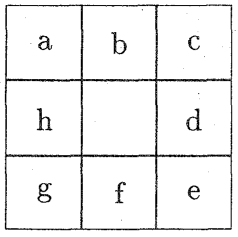
\includegraphics[scale=0.5]{img/jKxBPc.png}
\caption{Prikaz poretka jedinica teksture u susjedstvu srednjeg piksela.}
\end{figure}

\textbf{Primjer dobivanja teksturne jedinice}

\begin{multicols}{2}

\begin{minipage}{\linewidth}
\centering
\begin{tabularx}{0.4\textwidth}{| X | X | X |}
\hline
62 & 20 & 41 \\ 
\hline
79 & 40 & 30 \\ 
\hline
130 & 40 & 10 \\
\hline
\end{tabularx}
\captionof{figure}{Susjedstvo V = \{40, 62, 20, 41, 30, 10, 40, 130, 79\}}
\end{minipage}

\begin{minipage}{\linewidth}
\centering
\begin{tabularx}{0.4\textwidth}{| X | X | X |}
\hline
2 & 0 & 2 \\ 
\hline
2 &  & 0 \\ 
\hline
2 & 1 & 0 \\
\hline
\end{tabularx}
\captionof{figure}{Jedinica teksture TU = \{2, 0, 2, 0, 0, 1, 2, 2\}}
\end{minipage}

\end{multicols}

\begin{center}
\(TU = 2 \cdot 3^0 + 2 \cdot 3^2 + 3^5 + 2 \cdot 3^6 + 2 \cdot 3^7 + 2 \cdot 3^8 = 6094\)
\end{center}

Nakon definicije jedinice teksture, lako je objasniti lokalnu binarnu značajku. 
LBP se izračunava na potpuno jednak način osim što postoje samo dvije vrijednosti 
(0 i 1) umjesto 3. Ovakav način predložen je od T. Ojale i drugih \footnote{\cite{ojala}}. Ovaj 
pristup je pogodniji jer postoji ukupno 28  = 256 različitih kombinacija LPB-a, 
odnosno toliko koliko ima i razina svjetline pa su zbog toga slike u sivim 
tonovima prigodne.


\begin{multicols}{2}

\begin{minipage}{\linewidth}
\centering
\begin{tabularx}{0.4\textwidth}{| X | X | X |}
\hline
1 & 1 & 1 \\ 
\hline
0 &  & 1 \\ 
\hline
0 & 0 & 1 \\
\hline
\end{tabularx}
\captionof{figure}{Susjedstvo nakon usporedbe s centralnim pikselom}
\end{minipage}

\begin{minipage}{\linewidth}
\centering
\begin{tabularx}{0.4\textwidth}{| X | X | X |}
\hline
71 & 171 & 190 \\ 
\hline
5 & 55 & 78 \\ 
\hline
24 & 12 & 78 \\
\hline
\end{tabularx}
\captionof{figure}{Susjedstvo V = \{55, 71, 171, 190, 78, 78, 12, 24, 5\}}
\end{minipage}

\end{multicols}

\[LBP = 2^0 + 2^1 + 2^2 + 2^3 + 2^4 = 31\]

U prethodnim primjerima razmatrano je susjedstvo udaljeno samo za 
jedan piksel, međutim, to ne mora uvijek biti tako. Moguće je 
definirati susjedstvo kao kružnicu radijusa, npr. 3, što za sobom 
povlači veći broj piksela koji sudjeluju u nastajanju LBP-a. 

\bigbreak

Primjer slike dimenzija 64x64 i primijenjenog LBP operatora na tu 
sliku s radijusom redom 1, 2 i 3.

\begin{figure}[ht]
\begin{subfigure}[b]{0.24\linewidth}
\centering
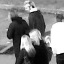
\includegraphics{img/1.jpg}
\end{subfigure}
\begin{subfigure}[b]{0.24\linewidth}
\centering

\includegraphics{img/2.jpg}
\end{subfigure}
\begin{subfigure}[b]{0.24\linewidth}
\centering

\includegraphics{img/3.jpg}
\end{subfigure}
\begin{subfigure}[b]{0.24\linewidth}
\centering

\includegraphics{img/4.jpg}
\end{subfigure}

\caption{Primjer dobivenih LBP slika iz izvorne slike uz različite radijuse oko centralnog piksela}
\end{figure}

Kao dodatno proširenje na osnovni operator LBP je takozvani jednolični uzorak 
(\textit{engl. uniform pattern}) koji može biti korišten za smanjenje dimenzija
vektora značajki, ali i kao jednostavni deskriptor otporan na rotaciju slike 
\footnote{\cite{barkan}}. Ideja je motivirana činjenicom da se neki 
binarni uzorci pojavljuju više od nekih drugih u slikama s teksturom. 
LBP se naziva jednoličnim ako ima najviše dvije 0-1 ili 1-0 tranzicije.
 Npr. 00010000 ima dvije tranzicije, ali 01010100 ima šest tranzicija 
 i on nije jednoličan. U izračunima LBP histograma, svaki uzorak ima 
 svoju grupu (poziciju), a svi koji nisu jednolični uzorci se 
 svrstavaju u zajedničku grupu. Koristeći jednolične uzorke,
  dimenzionalnost vektora značajki možemo smanjiti sa 256 na 59 
  (toliko ima jednoličnih uzoraka ako koristimo radijus jedan piksel).

\newpage

\subsection{Matrica pojavnosti sivih razina}

Dotična matrica predložena je od strane Haralicka i dr. \footnote{\cite{haralick}}, 
a Marana \footnote{\cite{marana}} je koristi za procjenu gustoće mnoštva.
Tipično se matrica izračunava nad crno bijelim slikama pa je poznatija
pod imenom matrica pojavnosti sivih razina (\textit{engl. Gray level co-occurence matrix - GLCM}).

\bigbreak

GLCM je statistička metoda procjene združenih uvjetnih vjerojatnosnih funkcija
gustoće \(f(i,j,d,\theta)\). Svaka \(f(i,j,d,\theta)\) predstavlja vjerojatnost 
da se par sivih razina \((i,j)\) javlja na udaljenosti \(d\) u smjeru \(\theta\)
na slici. Korištenje izvorne matrice u učenju različitih sustava klasifikacije 
je nepraktično jer sadrži veliku količinu informacije pa se zbog toga koriste
Haralickove značajke koje su prikazane u dodatku A.

\bigbreak

Primjer računanja funkcije gustoće vjerojatnosi za \(d=0, \theta=0\). Slika 
sa sivim razinama koja služi za izračunavanje funkcije \(f(i,j,1,0)\) nalazi 
se na slici 2.7.

\bigbreak
\bigbreak

\begin{minipage}{\linewidth}
\centering
\begin{tabularx}{0.3\textwidth}{| X | X | X | X |}
\hline
0 & 0 & 1 & 1 \\ 
\hline
0 & 0 & 1 & 1 \\ 
\hline
0 & 2 & 2 & 2 \\
\hline
2 & 2 & 3 & 4 \\
\hline
\end{tabularx}
\captionof{figure}{Primjer crno bijele slike}
\end{minipage}

\bigbreak

Postupak dobivanja elemenata matrice \(f(i,j,1,0)\) opisan je u sljedećim koracima i zatim
je prikazan izgled same matrice i izgled kada je provedena normalizacija matrice. 
Uzmimo da indeksi počinju od 0 i kao primjer
element \((0,0)\) koji predstavlja sva pojavljivanje dviju nula na udaljenosti 1
u smjeru od 0 stupnjeva, odnosno udesno. Iz slike je vidljivo da postoje takva
dva mjesta: prvi i drugi redak. Stoga se u matricu \(f(i,j,1,0)\) na mjestu
s indeksom \((0,0)\) upisuje broj 2. 

\bigbreak

Kao sljedeći element uzmimo \((2,3)\).
Potrebno je pronaći gdje se u izvornoj slici nalaze sive razine intenziteta
2 i 3 jedna kraj druge na udaljenosti 1 udesno. Iz slike je vidljivo da 
jedino mjesto pojave takvih razina u zdanjem retku, stoga u \(f(i,j,1,0)\)
na mjestu s indeksima \(2,3\) upisujemo 1. 

\newpage

Daljnjim nastavkom istog postupka
dolazi se do krajnjeg oblika matrice \(f(i,j,1,0)\) koja izgleda ovako

\begin{minipage}{\linewidth}
\centering
\[
\begin{bmatrix}
2&2&1&0\\
0&2&0&0\\
0&0&3&1\\
0&0&0&1\\
\end{bmatrix}
\quad
\quad
\begin{bmatrix}
0.167&0.167&0.083&0\\
0&0.167&0&0\\
0&0&0.25&0.083\\
0&0&0&0.083\\
\end{bmatrix}
\]
\captionof{figure}{Prikaz GLCM prije i nakon normalizacije}
\end{minipage}

Prikazana GLCM je oblika \(4,4\) jer sive razine izvorne slike mogu poprimiti
4 različit vrijednosti. U radu se koriste slike zapisane u 8-bitnom formatu
što znači da se veličina matrice povećava na \(256,256\) jer svaki piksel može
poprimiti jednu od 256 različitih vrijednosti. Zbog veličine matrice mnoge
kombinacije razina piksela se često ne pojavljuju u izvornim slikama što
dovodi do toga da su matrice dosta prazne, odnosno puno indeksa imaju popunjene 
nulama.

\bigbreak

\underline{\textbf{Primjer}}

Dobivanje vrijednosti Haralickove značajke - energija. Uzmimo izvornu sliku.
Energija se računa prema
\[
f_1 = \sum_{i}\sum_{j}p(i,j)^2
\]

gdje \(p(i,j)\) označava vrijednost GLCM za udaljenost 1 i kut od 0 stupnjeva.

\[
f_1 = 3 \cdot 0.167^2 + 3 \cdot 0.083^2 + 0.25^2 = 0.166834
\]

U ovom radu se koristi matrica naziva LBPCM(\textit{engl. Local binary pattern co-occurence matrix})
koja je u suštini GLCM samo što se izračnavanje vriijednosti matrice 
radi nad slikom sivih razina nad kojom je primjenjen operator LBP.

\newpage

\subsection{Klasifikator \textit{k} najbližih susjeda - \textit{k}-NN}

Ovaj klasifikator je jednostavan nadziran(\textit{engl.} supervised)
algoritam strojnog učenja koji može biti korišten za klasifikaciju
i regresije. Problemi klasifikacije imaju kao izlaz diskretne vrijednosti
dok s druge strane problemi regresije na izlazu poprimaju realne vrijednosti.
\textit{k}-NN algoritam pretpostavlja da se slične stvari nalaze 
jedne blizu drugih.

\bigbreak

Nadzirani algoritmi strojnog učenja oslanjaju se na označene početne uzorke
podataka kako bi dobili(naučili) funkciju koja daje prikladnu izlaznu vrijednost
kada joj se preda neki, još do sada neviđeni, uzorak. 

\bigbreak

Primjer problema 
za koji bi mogli iskoristiti ovakav mehanizam je učenje male koje su boje
objekti predočeni ispred nekakve vrste kamere, primjerice mobitela. Dijete
bi usmjerilo kameru u neki objekt koji bi bio u fokusu i kao povratnu informaciju,
aplikacija bi ispisala boju. Taj ispis bio bi pripadnost objekta nekom od predefiniranih 
razreda, npr. nekoliko različitih boja. Aplikacija bi izvukla 
dio slike oko fokusiranog objekta, nekim funkcijama obrade slike stvorila
vektor značajki i predala \textit{k}-NN klasifikatoru te bi on kao izlaz dao 
neku labelu. 

\bigbreak

Slovo \textit{k} u nazivu \textit{k}-NN predstavlja broj susjeda koji sudjeluju
u "glasanju". To glasanje predstavlja dodjeljivanje labele od strane \textit{k}
najbližih susjeda. Ukiliko je \(k=1\), labelu određuje samo najbliži susjed,
ako je \(k=3\), razred s više glasova pobjeđuje te se kao labela novome, dosad
nevđenome uzorku, dodjeljuje baš taj razred. Za broj susjeda se odabire pozitivan
broj koji je tipično malen. Kako bi odabrali dobru vrijednost broja \textit{k} poželjno
je algoritam pokrenuti nekoliko puta. 

\begin{multicols}{2}

Smanjenjem broja \textit{k} odluke postaju
sve nestablinije, npr. ako postoji jedan primjer nekog drugog 
razreda(koji previše odskače od vrijednosti svoga razreda) u blizini suprotnog razreda, 
može doći do krive klasifikacije što bi se inače izbjeglo povećanjem broja \textit{k}. 
Crna točka iz slike 2.9. prikazuje još neklasificiran uzorak. 

\begin{minipage}{\linewidth}
\vspace{10pt}
\centering
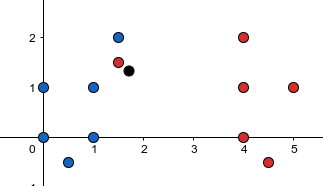
\includegraphics[width=0.8\linewidth]{img/krivo.png}
\captionof{figure}{Prikaz dva razreda s jednim nestandardnim uzorkom}
\end{minipage}

\end{multicols}

\bigbreak
Ukoliko bi kao konstantu \textit{k} izabrali 1, novi uzorak bi se klasificirao 
u crveni razred, a iz slike je jasno vidljivo da to nije poželjno. Točnost 
klasifikacije nije samo uvjetovana izborom konstante \textit{k}. Naime, 
ako su grupe pojedinih razreda raštrkane, odnosno njihov oblik je nepravilan,
točnost klasifikacije se narušava. Uspješnost algoritma može biti 
značajno degradirana korištenjem nekih značajki u vektorima koje ne 
doprinose međusobnoj diskriminaciji pojedinih vektora ili su skale pojedinih 
komponenti vektora neprilagođene njihovoj značajnosti pa je njihov ukupan doprinos prevelik. 

\bigbreak

\underline{\textbf{Primjer} - Klasifikacija \textit{k}-NN klasifikatorom.} \newline

Raspored uzoraka prikazan je na slici 2.10. Postoje 2 razreda - crveni i plavi. 
Uzorak koji se pokušava klasificirati označen je crnom bojom. 

\begin{minipage}{\linewidth}
\vspace{10pt}
\centering
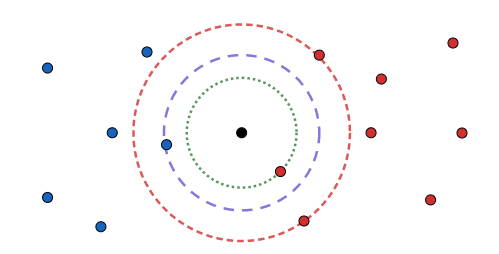
\includegraphics[width=0.8\linewidth]{img/klas.png}
\captionof{figure}{Prikaz uzoraka dva razreda i novog uzorka za klasifikaciju}
\end{minipage}

\bigbreak

Odabirom konstante \textit{k} utječemo na krajnju dodjelu labele.

\begin{itemize}
	\item \(k=1\) - Slučaj je prikazan crtkanom kružnicom zelene boje(kružnica najmanjeg 
	radijusa). Pripadnost se određuje na temelju najblžeg susjeda pa labela
	novog uzorka postaje crveni razred.
	\item \(k=2\) - Najbliža dva susjeda. Slučaj je prikazan plavom crtkanom kružnicom.
	Ovakva situacija nije poželjna jer se unutar granica nalazi jednak 
	broj pripadnika svakog od razreda. Kako bi razrješili situaciju mogli bi uzeti
	kao dodatnu mjeru udaljenost svakog od uzorka unutar kružnice do novog uzorka te
	pridodijeliti labelu bližeg. Kako bi izbjegli ovakve situacije dobra je praksa 
	uzimati neparne vrijednosti konstante \textit{k}.
	\item \(k=3\) - Situacija označena kružnicom najvećeg radijusa. Vidljivo
	je da su većinski pripadnici crvenog razreda unutar granica pa se
	novome uzorku dodjeljuje labela crvenog razreda.
\end{itemize}

\newpage

\subsection{Stroj s potpornim vektorima(\textit{engl.} Support vector machine) - SVM}

Ovaj klasifikator pripada vrsti linearnih klasifikatora što znači da 
ako postoji neki skup vektora X u kojem svaki od vektora \(x_i, i = 0, 1, ..., N\), 
pripada jednom od razreda \(\omega_1\) ili \(\omega_2\) te su ti razredi odvojivi hiperravninom 
u prostoru dimenzionalnosti \(N\). Cilj klasifikatora je izgraditi hiperravninu 
\(g(x) = \omega^Tx+\omega_0=0\).

%slika linearnih razreda
\begin{figure}[htbp]
\centering
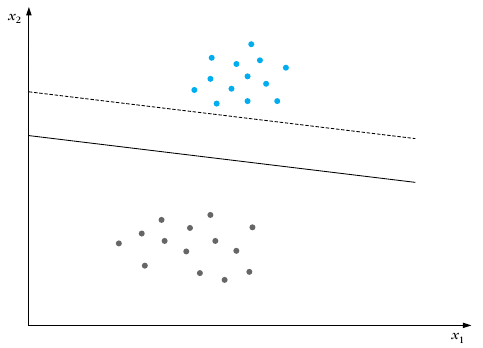
\includegraphics[scale=0.5]{img/linearniklasifikator.png}
\caption{Prikaz  dviju mogućih hiperravnina između dva razreda}
\end{figure}

Obje hiperravnine mogu poslužiti za odjeljivanje prikazanih razreda, međutim, 
uvijek je poželjnije imati čim otporniji klasifikator. Značenje otpornosti je u 
sljedećem. Ako se pojavi neki vektor koji je imalo ispod crtkane linije, 
klasificira se kao razred sivih točaka iako to ne bi bio slučaj malo pomnijim 
gledanjem slike. Cilj klasifikatora je izgraditi hiperravninu koja odjeljuje dva 
razreda, ali istovremeno ta hiperravnina mora biti što udaljenija od oba razreda 
čime se postiže otpornost klasifikatora na vektore koji malo odskaču od svojih razreda, 
bilo radi neke vrste šuma ili čega drugoga. 

Svaka hiperravnina je određena svojim smjerom (određeno s \textit{w}) i mjestom u prostoru (određeno s \(w_0\)). 
Pošto ne bismo željeli favorizirati niti jednu ravninu, trebamo odabrati jednu koja je 
jednako udaljena od odgovarajućih najbližih točaka razreda \(\omega_1\) i \(\omega_2\).  Odabrane hiperravnine 
označene su crnim linijama na slici 2. Margina udljenosti 1 je 2\(z_1\), a udaljenosti 2 je 2\(z_2\). 
Cilj je pronaći smjer koji daje maksmalnu moguću marginu. Margina je najmanja udaljenost 
između nekog vektora \(x_i\) i hiperravnine.

%slika s granicama
\begin{figure}[htbp]
\centering
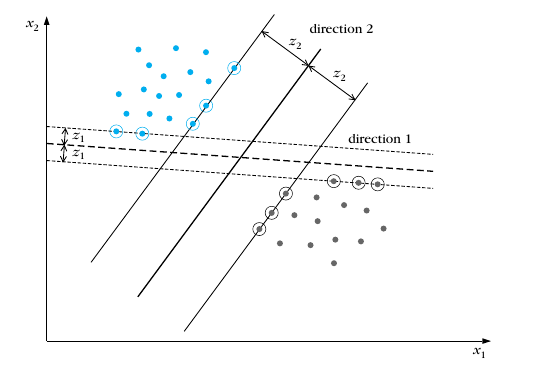
\includegraphics[scale=0.5]{img/slika10.png}
\caption{Prikaz potencijalnih hiperravnina koje dijele najbliže točke razreda}
\end{figure}

Želimo postići da je vrijednost \(g(x)\) u blizini najbliže točke jednaka 1 za razred \(\omega_1\), a
-1 za razred \(\omega_2\) što je moguće zapisati na sljedeći način

\begin{equation}
y_i(w^Tx_i + w_0) \ge 1, i = 1,2,...,N
\end{equation}

Kako bi dobili udaljenost dviju margina uzmimo jedan vektor \(x_p\) koji označava 
vektor iz središta koordinatnog sustava do neke točke na margini plavih točaka i 
drugi vektor \(x_s\) koji označava vektor iz središta koordinatnog sustava do neke točke 
na margini sivih točaka. Razlika tih dvaju vektora je vektor \(v_{ps}\). Umnožak vektora 
\(v_{ps}\) i jediničnog vektora dao bi udaljenost između dviju margina. Kako bi dobili 
jedinični vektor možemo podijeliti vektor  njegovom apsolutnom vrijednošću \(\left| \left| w \right| \right|\). 

\bigbreak

Umnoškom vektora \(v_{ps}\) i jediničnog vektora dobiva se \(\frac{2}{\left| \left| w \right| \right|}\).
Kako bi maksimizirali udaljenost između margina, moramo minimizirati \(\left| \left| w \right| \right|\). 
Kao funkciju minimizacije uzimamo \(\frac{1}{2}\left| \left| w \right| \right|^2\) radi dobrih matematičkih
svojstava.Za pronalazak minimuma uz ograničenja (1) možemo koristiti Lagrangeove multiplikatore. 



Funkcija optimizacije se pretvara u

\begin{equation}
L = \frac{1}{2}\left| \left| w \right| \right|^2 - \sum_i \alpha_i \left[y_i \left(w \cdot x_i + w_0\right) - 1\right]
\end{equation}

Za dobivanje ekstrema (2.2) potrebno je derivirati i izjednačiti s 0.

\[
\frac{\partial L}{\partial w} = w - \sum_i \alpha_i y_i x_i = 0
\]

\begin{equation}
w = \sum_i \alpha_i y_i x_i
\end{equation}

\[
\frac{\partial L}{\partial w_0} = w - \sum_i \alpha_i y_i = 0
\]

\begin{equation}
\sum_i \alpha_i y_i = 0
\end{equation}

\bigbreak

Uvrštavanjem (2.3) i (2.4) u (2.2) dobiva se sljedeće

\begin{equation}
L = \sum_i \alpha_i - \frac{1}{2} \sum_i \sum_j \alpha_i \alpha_j y_i y_j x_i^T \cdot x_j
\end{equation}

uz uvjet

\[
\sum_i \alpha_i y_i = 0
\]

čime se dobiva krajnji izraz koji je potrebno maksimizirati po \(\alpha\) nekim optimizacijskim
algoritmom. Iz izraza je vidljivo da njegova maksimizacija ovisi o umnošku parova početnih uzoraka. 
Jednom kada se Lagrangeovi multiplikatori izračunati, optimalna hiperravnina se dobiva 
uvrštavanjem u (2.3). Prikazani postupak optimizacije vrijedi i daje dobre rezultate u slučaju 
kada su razredi linearno odvojivi, u slučaju kada nisu postupa se drugačijim pristupom problemu.

\begin{multicols}{2}
Slučaj kada nisu razredi linearno odvojivi prikazan je na slici 3. Koliko god se trudilil nikako 
nije moguće pravcem odijeliti dva razreda kako se ne bi događala kriva klasifikacija nekih 
budućih uzoraka. Ideja je prijeći u neki viši dimenzijski sustav u nadi da će razredi postati 
linearn odvojivi. Uzmimo kao primjer sliku 2.3 i prijeđimo u trodimenzionalni sustav. 

\bigbreak

Novonastala situacija prikazana je na slici 2.4. U ovoj dimenziji granica koja dijeli razrede uzoraka 
postaje ravnina. Vidimo da je u prostoru s ovom dimenzionalnošću moguće odijeliti uzorke jedne 
od drugih tako da ne postoje preklapanja dvaju razreda koja bi rezltirala krivom klasifikacijom.
Granica koja dijeli dva razreda prikazana je zelenkastom bojom na slici 2.4.

\begin{minipage}{\linewidth}
\vspace{10pt}
\centering
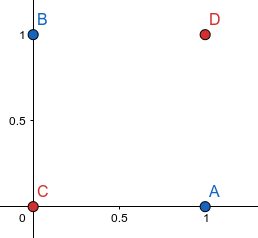
\includegraphics[width=0.8\linewidth]{img/neseparabilni.png}
\captionof{figure}{Linearno nerazdvojivi razredi}
\end{minipage}

\begin{minipage}{\linewidth}
\vspace{10pt}
\centering
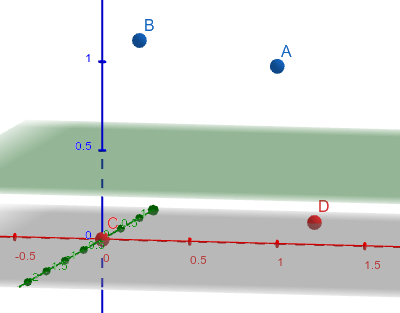
\includegraphics[width=0.8\linewidth]{img/3d.png}
\captionof{figure}{Linearno nerazdvojivi razredi u većoj dimenziji postaju linearno odvojivi}
\end{minipage}
\end{multicols}

Funkcija kojom se prelazi u drugu dimenziju označava se s \(\varphi(x)\). Kako bi se navedena ideja
koristila u funkciji koja se maksimizira, dovoljno je samo napraviti sljedeće
jer funkcija ovisi samo o polaznom skupu uzoraka, odnosno \(X\).

\[
L = \sum \alpha_i - \frac{1}{2} \sum_i \sum_j \alpha_i \alpha_j y_i y_j \varphi(x_i) \cdot \varphi(x_j)
\]

Kraći zapis zapis korišten za \(\varphi(x_i) \cdot \varphi(x_j)\) je \(k(x_i, x_j)\) čime se označavaju 
jezgrene funkcije. Jezgrene funkcije služe za preslikavanje uzoraka iz početne, relativno niske 
dimenzionalnosti, u višu, moguće puno veću dimenzionalnost od izvorne kako bi uzorci u višoj 
dimenzionalnosti bili linearno odvojivi.

\begin{table}[htbp]
\centering
\caption{Prikaz nekih popularnih jezgara}
\begin{tabular}{ll}
\hline
ime & formula \\ \hline
Linearna: & \(K\left( x_i, x_j\right) = x_i^Tx_j\) \\
Polinomna: & \(K\left( x_i, x_j\right) = \left( a \cdot x_i^Tx_j + b\right)^d\)  \\
RBF: & \(K\left( x_i, x_j\right) = e^{-\frac{\left\lVert x_i - x_j \right\rVert^2}{\sigma^2}}\) \\
Sigmoida: & \(K(x_i, x_j) = tanh\left( \sigma x_i^T x_j + r\right)\) \\
Potencija: & \(K\left( x_i, x_j\right) = -\left\lVert x_i - x_j\right\rVert^\beta\) \\
Logaritam: & \(K\left( x_i, x_j\right) = -log\left( 1 + \left\lVert x_i - x_j\right\rVert^\beta\right)\) 
\end{tabular}
\end{table}

Ova inačica SVM-a namijenjena je klasifikaciji gdje samo postoje 2 razreda. Međutim, 
jedan problem s više razreda može se podijeliti u više manjih binarnih problema klasifikacije. 
Popularne metode su: 

\begin{itemize}
	\item jedan protiv svih gdje se labela uzorku dodijeljuje prema klasifikatoru koji 
	ima funkciju najveće vrijednosti 
	\item jedan protiv drugog gdje se uzorak klasificira prema strategiji najvećeg 
	broja pobjedi što znači da svaki od klasifikatora pridjeljuje pripadnost jednom od razreda i razred s najviše glasova pobjeđuje
\end{itemize}

\newpage

\subsection{Gradijent slike}

Gradijent slike je promjena intenziteta ili boje u nekom smjeru na slici.

\begin{figure}[htbp]
\centering

\includegraphics[width=0.8\linewidth]{img/Gradient2.png}
\caption{Prikaz smjera gradijenta plavim strelicama, tamnija boja označava veće vrijednosti.}
\end{figure}

%\footnote{\cite{wikiGradient}}

Matematički, gradijent je funkcija dviju varijabli, vektor s dvije komponente koje su dobivene
derivacijom u horizontalnom i vertikalnom smjeru. Na svakom pikselu vektor gradijenta je smjer 
najveće promjene intenziteta, a duljina toga vektora odgovara brzini promjene u tom smjeru.

\[
\nabla f = \left[ \begin{array}{c} g_x \\ g_y \end{array}\right]
 = \left[ \begin{array}{c} \frac{\partial f}{\partial x} \\ \frac{\partial f}{\partial y} \end{array}\right]
 \textrm{, a iznos je dan s  } \sqrt{g_x^2 + g_y^2}
\]

\bigbreak

Kako je funkcija intenziteta slike pozanta samo u diskretnim točkama, derivacija ove funkcije 
ne može biti definirana ako se ne pretpostavi da iza svega toga leži kontinuirana funkcija 
intenziteta koja je uzorkovana u dotičnim pikselima. Aproksimacije ovih funkcija derivacije 
mogu biti definirane s različitim stupnjevima točnosti. Jedan od popularnih načina za 
aproksimaciju gradijenta slike je konvolucija slike s nekom jezgrom, primjerice sa Sobelovim operatorom.

\newpage

\subsection{Sobelov operator}

Ovaj operator koristi dvije 3 \(\times\) 3 jezgre koju su konvolirane s izvornom slikom kako bi se aproksiirale 
derivacije – jedna za x smjer, a druga za y smjer. Označimo izvornu sliku kao dvodimenizonalnu matricu \(A\), sliku
koja je dobivena konvolucijom jezgre za x smjer i slike \(A\) kao \(G_x\), a sliku koja je dobivena konvolucijom 
jezgre za y smjer i slike \(A\) s \(G_y\).

\[G_x = 
\begin{bmatrix} 
1 & 0 & -1\\ 
2 & 0 & -2\\ 
1 & 0 & -1 
\end{bmatrix}
 * A
  \quad\quad\quad
 G_y = 
\begin{bmatrix} 
 1 & 2 & 1\\ 
 0 & 0 & 0\\ 
 -1 & -2 & -1
\end{bmatrix}
 * A
\]
\bigbreak
gdje * označava operaciju konvolucije, a krajnja slika se dobije na sljedeći način 
\[
G = \sqrt{G_x^2 + G_y^2}
\].

{\large\textbf{Primjer Sobelovog operatora}}

\begin{multicols}{2}

\begin{minipage}{\linewidth}
\centering
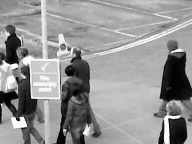
\includegraphics[width=0.8\linewidth]{img/2982.jpg}
\captionof{figure}{Izvorna slika}
\end{minipage}

\begin{minipage}{\linewidth}
\centering
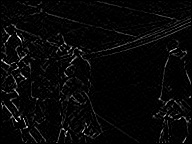
\includegraphics[width=0.8\linewidth]{img/sobel.jpg}
\captionof{figure}{Prijenjen Sobelov operator na izvornoj slici}
\end{minipage}

\begin{minipage}{\linewidth}
\centering
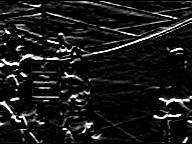
\includegraphics[width=0.8\linewidth]{img/sobely.jpg}
\captionof{figure}{Prijenjen Sobelov operator u smjeru y na izvornoj slici}
\end{minipage}

\begin{minipage}{\linewidth}
\centering
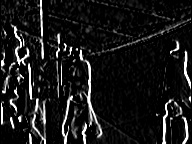
\includegraphics[width=0.8\linewidth]{img/sobelx.jpg}
\captionof{figure}{Prijenjen Sobelov operator u smjeru x na izvornoj slici}
\end{minipage}

\end{multicols}

\newpage

\subsection{Haralickove značajke}

Početna pretpostavka u karakterizaciji teksture slike je da 
matrica pojavnosti sivih tonova sadrži svu  informaciju o teksturi slike. 
Samim time sve teksturne značajke će se izračunavati iz matrice pojavnosti sivih 
tonova. Funkcije koje definiraju skup od 14 mjera teksturnih značajki dane se ispod. 
Neke od tih mjera se odnose na specifične teksturne karakteristike poput homogenosti, 
kontrasta i prisutnosti grupiranih ili usmjerenih struktura unutar slike. Druge mjere 
opisuju složenost i način promjene sivih tonova unutar slike. Iako te mjere sadrže 
informaciju o teksturnim značajkama slike, teško je identificirati koja je teksturna 
značajka karakterizirana nekom konkretnom funkcijom. Definicije sljedećih funkcija preuzete su
iz izvornog rada Haralicka i drugih. \footnote{\cite{haralick}}






\chapter{Opis postupka}

Predlaže se tehnika klizećeg prozora za klasifikaciju i lociranje područja
mnoštva. Pripremne radnje obuhvaćaju pretvorbu izvornih slika, dimennzija
768 x 576, u sive tonove i dijeljenje njih samih u manje podslike, dimenzija
192 x 144, kojih ima 16 po svakoj izvornoj slici. Svaka podslika varira
po gustoći mnoštva, pozadini i uvjetima osvjetljenja.  


\begin{figure}[ht]
	\begin{subfigure}[b]{0.19\linewidth}
		\centering
		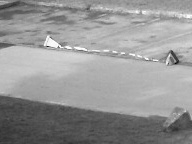
\includegraphics[scale=0.5]{img/noflow.jpg}
		\caption{No flow}
	\end{subfigure}
	\begin{subfigure}[b]{0.19\linewidth}
		\centering
		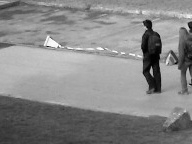
\includegraphics[scale=0.5]{img/freeflow.jpg}
		\caption{Free flow}
	\end{subfigure}
	\begin{subfigure}[b]{0.19\linewidth}
		\centering
		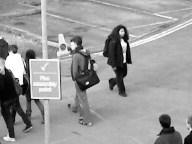
\includegraphics[scale=0.5]{img/restrictedflow.jpg}
		\caption{Restricted flow}
	\end{subfigure}
	\begin{subfigure}[b]{0.19\linewidth}
		\centering
		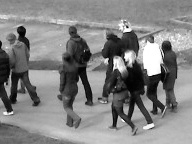
\includegraphics[scale=0.5]{img/denseflow.jpg}
		\caption{Dense flow}
	\end{subfigure}
	\begin{subfigure}[b]{0.19\linewidth}
		\centering
		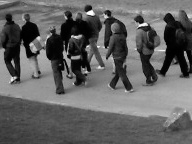
\includegraphics[scale=0.5]{img/jammedflow.jpg}
		\caption{Jammed flow}
	\end{subfigure}
\caption{Prikaz pojedinih gustoća mnoštva}
\end{figure}

Sve se podslike ručno označene pripadnim razredima gustoće prema
\footnote{\cite{polus}} uz dotadnu oznaku \enquote{no flow} koja 
predstavlja podslike u kojima nema nikakvog mnoštva. Sljedeće se primjenjuje
operator LBP nad svakom podslikom. Nakon dobivanje slike lokalnih binarnih 
značajki, koristeći se tenhnikom kliznog prozora, konstruira se matrica 
pojavnosti lokalnih binarnih značajki(LBPCM) nad svakim oknom podslike. 
Iz svake LBPCM izračunavaju se željene Haralickove značajke i te se vrijednosti
pohranjuju u vektor značajki. Vektor značajki se sastoji od vrijednosti
Haralickovih značajki svakog okna, odnosno vektor značajki neke podslike 
sastoji se od vrijednosti Haralickovih značajki njezinih okna. Po završteku 
stvaranja, vektori značajki, se predaju \textit{k}-NN klasifikatoru ili SVM-u.

\bigbreak

Na kraju se pristupa evaluaciji samih klasifikatora i eventualnoj izmjeni
saih parametara nadi boljeg rezultata u sljedećoj iteraciji učenja. Za učenje
klasifikatora korisiti se \(70\%\) izvornih slika, a za testiranje ostatak.

\bigbreak

Cijeli sustav podijeljen je u dva dijela koji se na kraju sjedinjavaju u 
jednu cjelinu. Prvi dio sastoji se od klasifikator koji služi samo za 
klasifikaciju slika sivih razina (klasifikator može biti \textit{k}-NN ili SVM)
dok drugi dio služi samo za klasifikaciju slika nad kojima se primjenjuje
operator gradijenta (klasifikator može biti \textit{k}-NN ili SVM).

\bigbreak

Sjedinjenje dvaju različitih klasifikatora obavlja se pomoću nove vrste
klasifikatora - glasačkog klasifikatora (\textit{engl. voting classifier}).
Ovakva vrsta klasifikatora pogodna je zbog načina na koji daje važnost pojedinim
klasifikatoru od kojih se sastoji. Na odluku klasifikatora može se utjecati
na više načina. Prvi je \enquote{tvrdo glasanje} (većinsko glasanje), gdje svaki od klasifikator glasa
za neku labelu, a najbrojnija labela pobjeđuje i dodjeljuje se novome uzorku 
koji se klasificira. Ovakvo glasanje je moguće i modificirati na način da 
se svakome klasifikatoru dodijeli neka težina, npr. ovisno o točnosti njegove
klasifikacije na setu slika za učenje.

\bigbreak

Drugi način je \enquote{meko glasanje} (\textit{engl. soft voting}) gdje
se dohvate vjerojatnosti klasifikacije svake labele svakog od klasifikatora,
uprosječe se, pa se na temelju tih novih vjerojatnosnih vrijednosti određuje
pripadnost dosad neviđenog uzorka. Pošto su poznate vjerojatnosti klasifikacije
moguće je množiti svaku vjerojatnost nekom težinom i time utjecati na ishod odluke.


\begin{center}

SLIKA ARHITEKTURE SUSTAVA

\end{center}

\chapter{Upute za korištenje i prikaz međukoraka}

rogramska podrška ovdje obrađivanog postupaka pisana je u Python 3.6 
programskom jeziku. Usto je potrebno instalirati dodatne Python 
knjižnice: OpenCV, scikit-learn i PIL.

Za pokretanje aplikacije putem grafičkog sučelja potrebno je kliknuti 
na app.py ili putem terminala upisati naredbu „python app.py“ iz 
vršnog direktorija projekta. Nakon što je aplikacija pokrenuta 
otvoren je sljedeći prozor. 

\begin{figure}[ht]
\centering
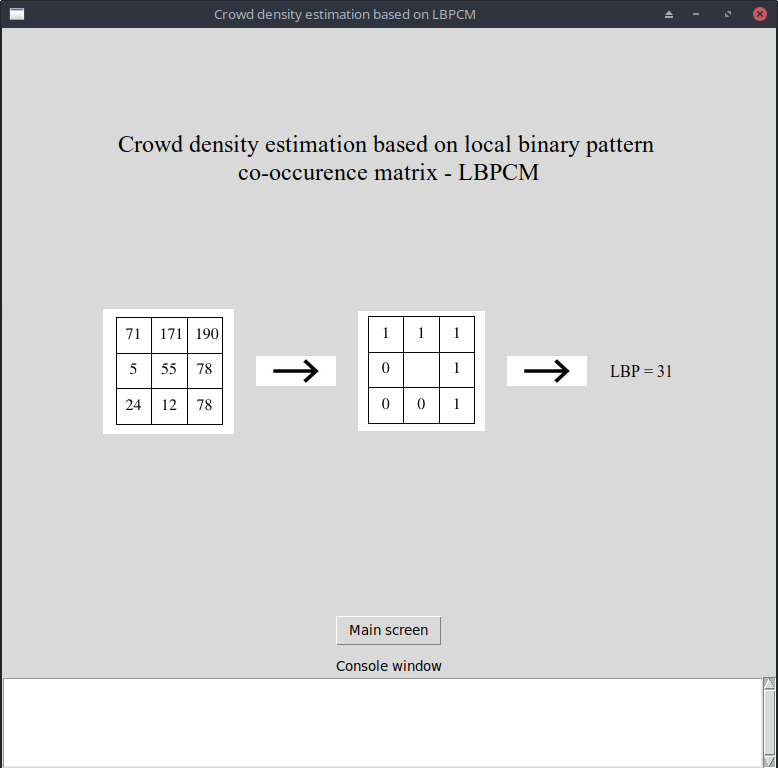
\includegraphics[scale=0.4]{img/startpage.png}
\caption{Prikaz početnog prozora nakon pokretanja aplikacije}
\end{figure}

Početni prozor prikazuje naziv rada na kojem se temelji ovaj završni rad, 
slikovni prikaz postupka lokalnih binarnih značajki i gumb \enquote{Main screen}
koji otvara stranicu s glavnim funkcionalnostima aplikacije. U podnožuju svakog
prozora nalazi se prazan prozor koji \enquote{Console window} koji ima ulogu
mjesta u koji se ispisuju važnije informacije poput upozorenja, eventualnih 
grešaka i rezultata izvođenja nekih drugih funkcija. Pritiskom na gumb \enquote{Main screen}
otvara se glavni prozor koji sadrži sve funkcionalnosti aplikacije.

\begin{figure}[ht]
\centering
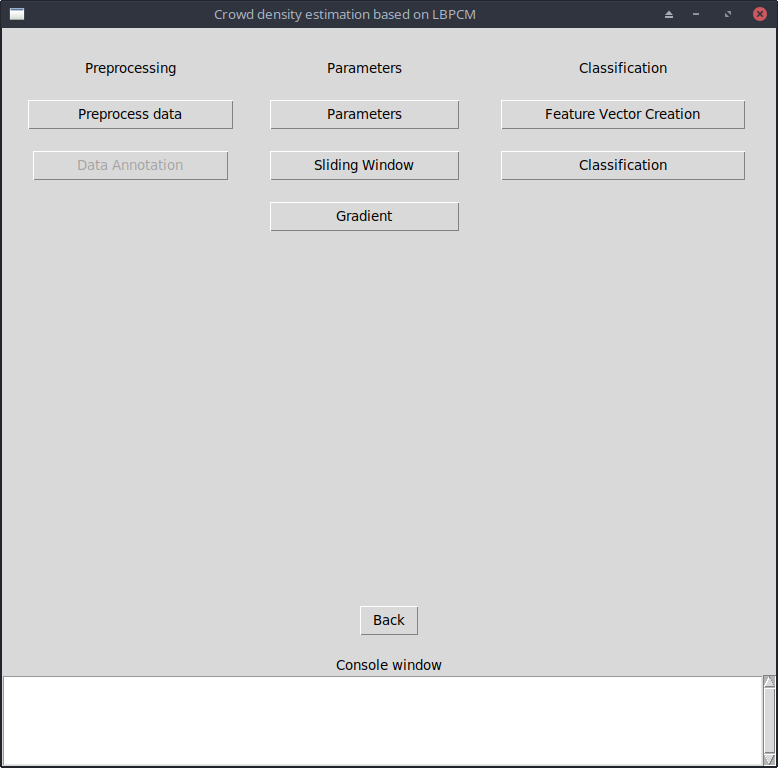
\includegraphics[scale=0.4]{img/mainscreen.png}
\caption{Prikaz glavnog prozora}
\end{figure}

Prostor glavnog prozora podijeljen je u tri dijela. Prvi dio se sastoji
od radnja koje je potrebno obaviti prije samog postupka učenja, a to su:
priprema izvornih slika podjelom u manje podslike i označavanje svake 
podslike odgovarajućim razredom gustoće mnoštva. Po završetku navedenih radnja
moguće je nastaviti s daljnjim postupkom.

\bigbreak

Drugi dio prozora služi za promjenu parametara aplkacije, uvid u tehniku 
klizećeg okna gdje je moguće vidjeti kako se mijenjaju iznosi Haralickovih značajki
prilikom putovanja klizećeg okna po pojedinoj slici i na kraju korištenje
opertora gradijenta na odabranoj slici.

\bigbreak

Zadnji dio prozora obuhvaća samu fazu stvaranja vektora značajki (učenje
klasifikatora) gdje se postavljaju svi parametri pojedinog modela i pokreće
postupak učenja i drugi dio koji je zaslužan za postupak klasifikacije
dosad neviđenih uzoraka nekim od već naučenih modela.


\subsection{Podjela slika u podslike}

Prije svega potrebno je pripremiti skup slika koji se koristi za učenje i 
kasnije za verifikaciju klasifikatora. Izvorni skup se sastoji od 221 slike
koje su izvučene iz video zapisa jedne nadzorne kamere. Svaka slika je dimenzija
768 x 576 te se podijeli u 16 jednakih podslika 192 x 144. Ova konkretna dimenzija
podslika je odabrana kako ne bi ostalo neiskorištenih piksela na rubovima i 
kako dimenzije novonastalih podslika ne bi previše odskakala od veličine mnoštva
koje je prisutno u izvornim slikama. Nakon što su slike podijeljene na manje dijelove,
novonastalih podslika ima 3536 koje se zatim pretvaraju u slike sivih razina kako
bi se prilikom računanja Haralickovih značajki tijekom učenja klasifikatora taj
korak mogao preskočiti pa bi se uštedjelo vrijeme. 

\bigbreak

Aplikacija nudi potporu za izvođenje navedenog postupka. Kako bi se izvorne
slike podijelile u manje podslike potrebno je pritisnuti na gumb \enquote{Preprocess data}
koji otvara stranicu sljedećeg izgleda.

\begin{figure}[ht]
\centering
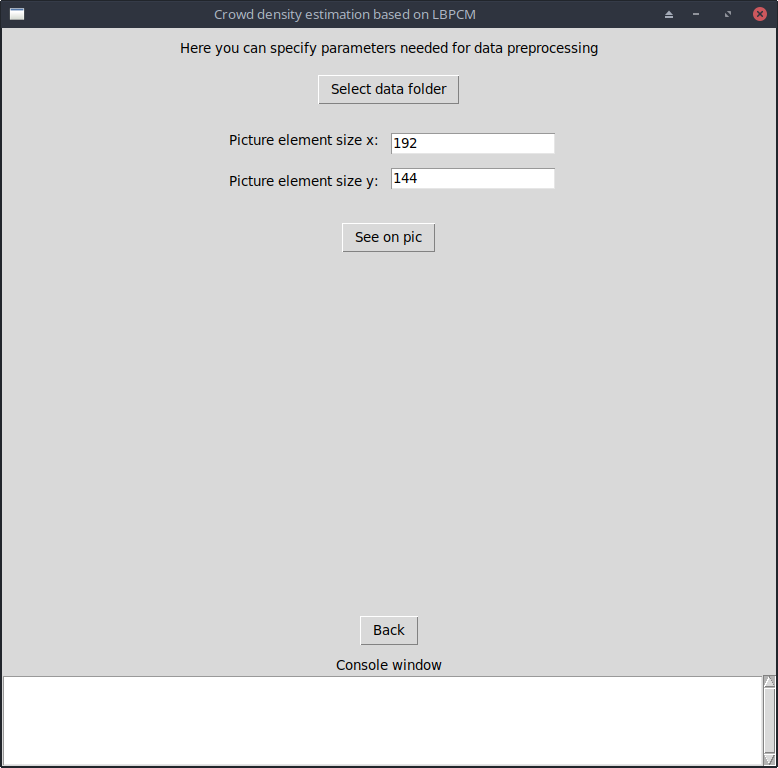
\includegraphics[scale=0.4]{img/preprocessdata.png}
\caption{Prikaz stranice za obradu izvornih slika}
\end{figure}

Prozor na samom vrhu ima gumb za odabir direktorija koji sadrži izvorne slike
za učenje i testiranje. Po odabiru navedenog direktorija mogu se upisati 
željene dimenzije podslika koje će nastati dijeljenjem izvorne slike.
Prvi element unosa sadrži veličinu s x smjeru, a drugi u y smjeru. Nakon
unešenih dimenzija moguće je vidjeti kako bi izgledale konkretne dimenzije
na izvornoj slici pritiskom na gumb \enquote{See on pic}. Nakon pritiska na gumb
pojavljuje se sljedeći dio prozora.

\begin{figure}[ht]
\centering
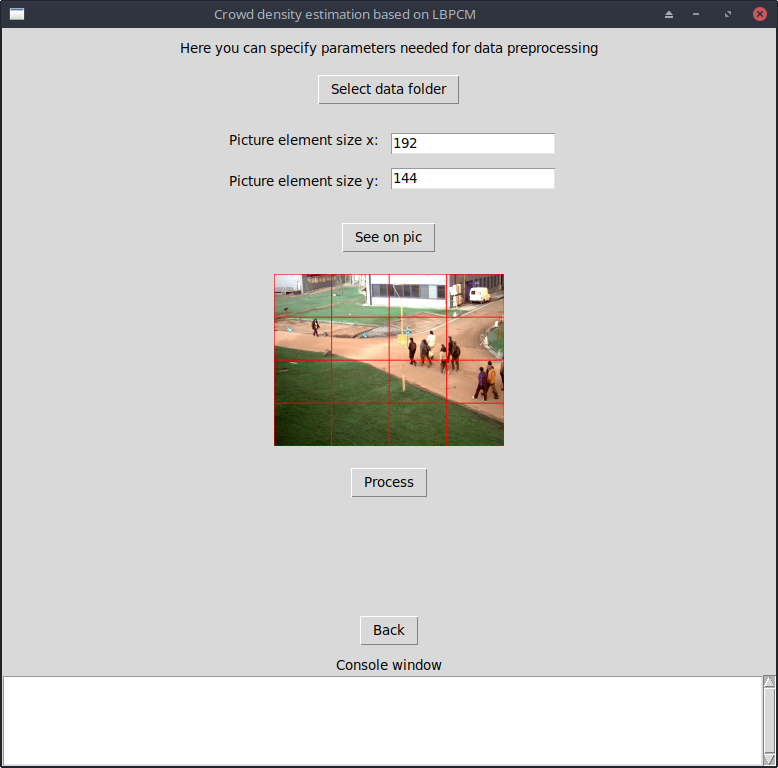
\includegraphics[scale=0.4]{img/seeonpic.png}
\caption{Prikaz izgleda podslike s nešenih dimenzijama}
\end{figure}

Novi dio prozora prikazuje jednu izvornu sliku iz odabranog direktorija
s podjelom na manje podslike koje su dimenzije unešene iznad. Svaka podslika
prikazana je crvenim linijama i ako nismo zadovoljni njihovom dimenzijom
moguće je upisati neke druge vrijednosti i vidjeti novi rezultat. Ukoliko 
nam odgovara veličina podslika potrebno je pritisnuti gumb \enquote{Preprocess}
koji pokreće postupak dijeljenja slika iz odabranog direktorija i zapisuje ih u 
direktorij \enquote{preprocessedData}. Taj direktorij nakon završenog postupka
sadrži 3536 podslika u sivim razinama, ukoliko su korištene dienzije 192 x 144, 
pa je moguće prijeću u sljedeću fazu, a to je označavanje svake pojedine podslike.

\newpage

\begin{figure}[ht]
\centering
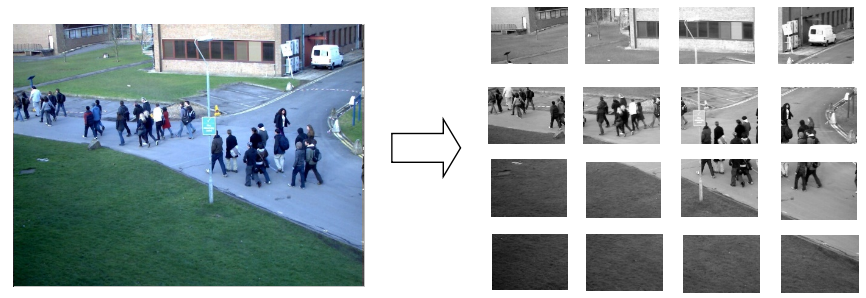
\includegraphics[scale=0.4]{img/splitted.png}
\caption{Prikaz podijeljene izvorne slika na manje podslike}
\end{figure}

\subsection{Označavanje podslika}

Po završetku dijeljenja izvornih slika u manje podslike pristupa se postupku
označavanja podslika. Kako bi mogli označiti svaku pojedinu podsliku na
što jednostavniji način potrebno je pritisnuti gumb \enquote{Data Annotation} 
u glavnom prozoru aplikacije. Nakon pritiska na gumb otvara se sljedeći prozor.

\begin{figure}[ht]
\centering
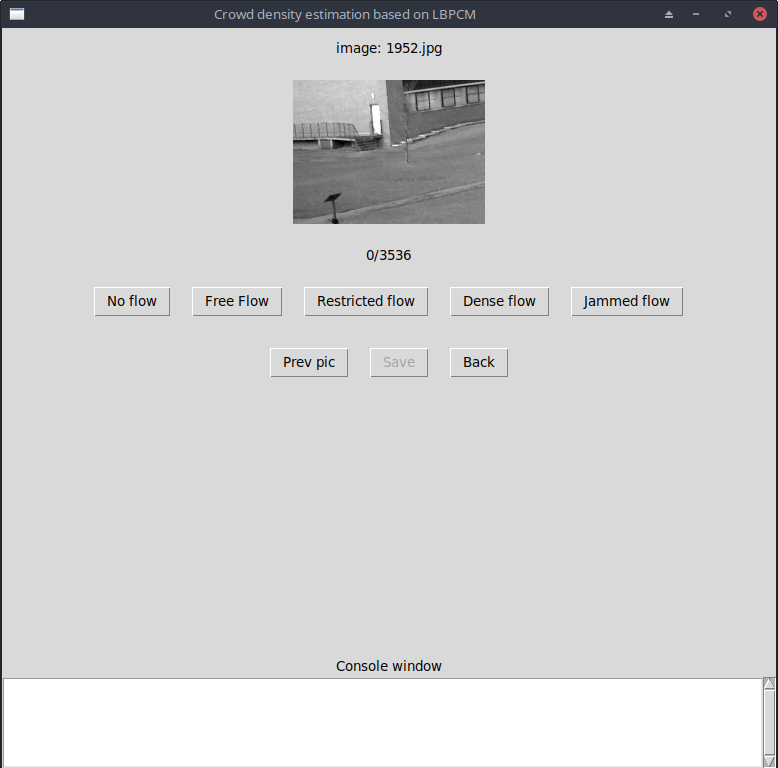
\includegraphics[scale=0.4]{img/dataannotation.png}
\caption{Prikaz prozora za označavanje podslika}
\end{figure}

Najgornji dio prozora prikazuje ime trenutne podslike koju je potrebno označiti.
Ispod naziva se nalazi konkretna slika koja se označava, a i prisutan je brojač
koji prikazuje broj označenih slika. Ispod brojača postoji 5 gumba koji
označavaju razine gustoće mnoštva. Podslika se označava pritiskom na jedan
od gumba koji odgovara gustoći mnoštva zatečenoj na trenutnoj slici. Nakon pritiska
na gumb pojavljuje se sljedeća od podslika koju je potrebno označiti, a labela
prethodne podslike se zapisuje u interni spremnik. 

\bigbreak

Nakon što su sve podslike označene
odgovarajućim labelama, interni spremnik je moguće spremiti na disk u obliku 
tekstualne datoteke pritiskom na gumb \enquote{Save}. Nakon pritiska na gumb
\enquote{Save} stvara se tekstualna datoeka imena \enquote{labeledData.txt}
, a svaki redak je oblika 0.jpg:2, gdje 0.jpg predstavlja ime podslike koje 
je jedinstveno, a 2 označava pripadni razred gustoće mnoštva. Ukoliko je 
došlo do pogreške prilikom označavanje neke podslike moguće je pritisnuti
gumb \enquote{Prev pic} čime se vraća prethodna slika kojoj je moguće pridijeliti
drugačiju labelu. Potebno je napomenuti da se jednom označene podslike ne trebaju 
više označavati prilikom svakog procesa učenja nekog klasifikatora nego 
je samo potrebno učitati postojeću datoteku.

\subsection{Stvaranje vektora značajki}

Jednom kada se slike podijeljene u manje podslike i nakon završetka označavanja
svih podslika, moguće je pristupiti postupku stvaranja vektora značajki. 
Kako bi pristupili tome prozoru, potrebno je pritisnuti gumb \enquote{Feature Vector Creation} 
nakon čega se otvara prozor prikazan na slici 4.7.

Prozor ne prikazuje puno osim broja podslika i informacije jesu li labele
podliska učitane u memoriju ili nisu. Kako bi ih učitali potrebno je pritusnuti
na gumb \enquote{Load labels} nakon čega se otvara prozor za odabir tekstualne datoteke
s labelama. Ako su labele uspješno učitane, mijenja se tekst ispod broja
podslika u tekst zelene boje \enquote{LOADED}. Podnožje prozora još sadrži gumb
za povratak na prethodnu stranicu i gumb za dodavanje novih konfiguracije koji će biti
ubrzo objašnjen. 

\bigbreak

Središnji dio prozora trenutno ne prikazuje ništa jer nije dodana niti jedna
konfiguracija. Jednom kada se doda nova konkfiguracija, u središnjom dijelu
prozora stvori se traka napretka koja prikazuje koliko još ima do završetka 
te pojedine konfiguracije. 

Stvaranju vektora značajki prethodi stvaranje neke konfiguracije. Kako bi se 
stvorila nova konfiguracija potrebno je pritisnuti na gumb \enquote{Add configurations}.
Nakon pritiska na gumb otvara se prozor prikazan na slici 4.8.

\newpage

\begin{minipage}{\linewidth}
\centering
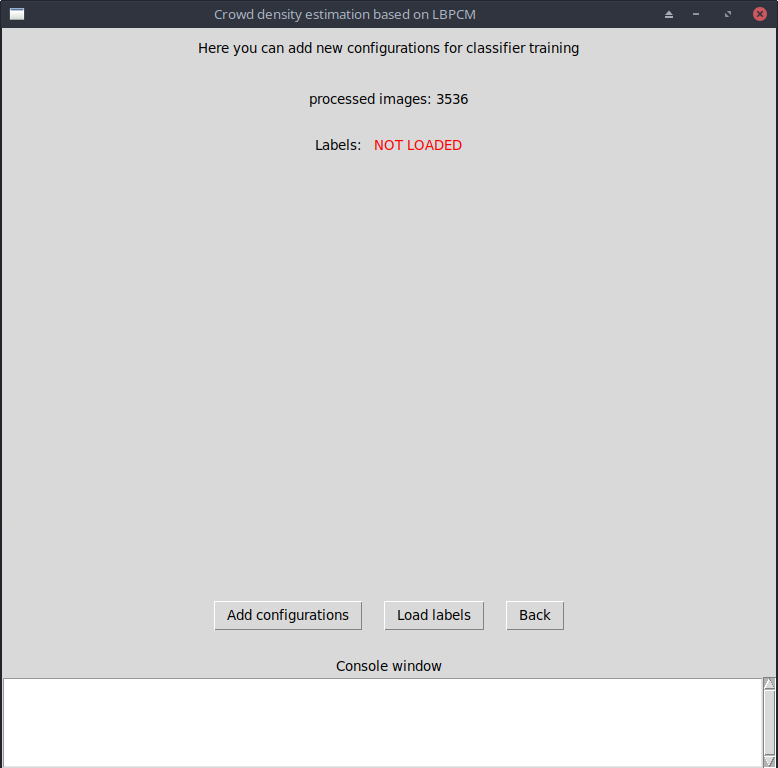
\includegraphics[scale=0.35]{img/fvc1.png}
\captionof{figure}{Početni prozor za stvaranje vektora značajki}
\end{minipage}

\bigbreak

\begin{minipage}{\linewidth}
\centering
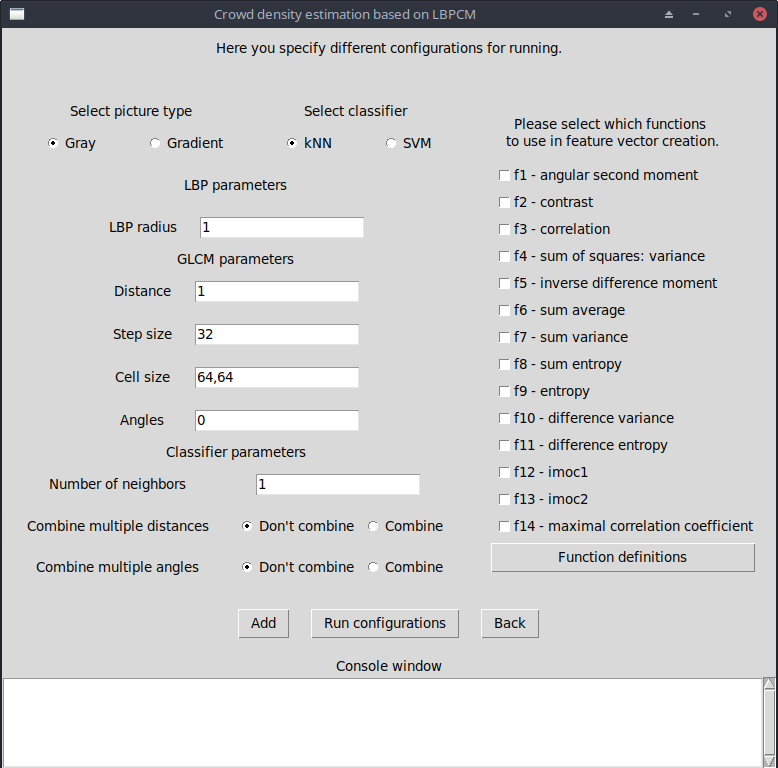
\includegraphics[scale=0.35]{img/fvc2.png}
\captionof{figure}{Izgled prozora za stvaranje konfiguracije}
\end{minipage}

\bigbreak

Prozor za stvaranje konfiguracije sastoji se od lijevog i desnog dijela. 
Lijevi dio služi za unos parametara dok je u desnom dijelu moguće odabrati
Haralickove značajke koje se izračunavaju iz GLCM. Na vrhu prozora potrebno
je odabrati vrstu slike nad kojom se primjenjuje LBP operator: sliku 
sivih razina (\textit{gray}) ili sliku sivih razina nad kojom je 
primijenjen operator gradijenta (\textit{gradient}). 

\bigbreak

Za odabir klasifikatora postoje dvije mogućnosti: \textit{k}-NN klasifikator i 
SVM. Odabranom klasifikatoru se prosljeđuju stvoreni vektori značajki gdje se onda
interno spreme u slučaju \textit{k}-NN ili upotrijebe u fazi učenja klasifikatora
u slučaju SVM. 

\begin{table}
\begin{tabular}{p{0.35\linewidth} | p{0.6\linewidth}}
Parametar & Opis \\
\hline
LBP radius & označava veličinu radijusa oko središnjeg piksela
na temelju kojeg se izračunava LBP neke slike \\

\\
\hline
Distance & predstavlja udaljenost u GLCM na temelju koje 
se gledaju pojavnosti sivih razina. Moguće je istovremeno izračunavati vrijednosti
za više udaljenosti, a u tom slučaju ih je potrebno odvojiti zarezom \\

\\
\hline
Step size & veličina koraka u x i y smjeru prilikom tehnike klizećeg okna \\

\\
\hline
Cell size & veličina putujućeg okna u smjeru x, y \\

\\
\hline
Angles & su svi kutovi za koje se konstruira GLCM, odvajaju
se zarezom i upisuju u stupnjevima \\

\\
\hline
Number of neighbors & koristi se kod \textit{k}-NN klasifikatora
gdje označava broj susjeda na temelju čijeg se glasanja daje labela novome uzorku \\

\\
\hline
Combine multiple distances & predstavlja opciju kombiniranja više
udaljenosti u jednu, npr. ako je GLCM izračunavana za udaljenosti 1, 2 i 3, matrice
se zbroje i podijele s 3 ako bi se odabrao slučaj s kombinacijom udaljenosti \enquote{combine}
u suprotnom se svaka interpretira za sebe \\

\\
\hline
Combine multiple angles & jednako kao i za udaljenosti

\end{tabular}
\caption{Opis parametara konfiguracije}
\end{table}

\bigbreak

Desna strana prozora prikazuje svih 14 Haralickovih značajki. Jednom kada 
su odabrani svi parametri s lijeve strane, desna strana se koristi za odabir 
značajki koje se izračunavaju prilikom kreiranja vektora značajki svake pojedine
konfiguracije. Svaka konfiguracija može imati broj značajki veći ili jednak jedan. 
Ovisno o broju odabranih značajki i broju različitih udaljenosti i kutova, vrijeme
stvaranja vektora značajki može biti značajno dugačko stoga se u fazi eksperimentiranja
stvara više konfiguracija koje se mogu izvoditi istovremeno ukoliko je računalo
višeprocesorsko. Definicije Haralickovih značajki moguće je vidjeti u Dodatku A
ili pritiskom na gumb \enquote{Function definitions} nakon čega se otvara novi
prozor u kojem je naveden algebarski oblik svake Haralickove značajke kao i 
opisi drugih oznaka korištenih u formulama. 

\bigbreak

Nakon odabira željenih Haralickovih
značajki moguće je pritisnuti na gumb \enquote{Add} čime se stvara
nova konfiguracija. Ukoliko želimo dodati još konfiguracija, potrebno je samo
označiti ili izmijeniti postojeće parametre i opet pritisnuti gumb \enquote{Add}.
Svakim pritiskom gumba stvara se nova konfiguracija i interno pohranjuje te čeka na
pokretanje postupka stvaranja vektora značajki. Kada smo dodali sve konfiguracije
koje želimo, za početak stvaranje vektora značajki potrebno je pritisnuti gumb
\enquote{Run configurations} čime se onoliko konfiguracije izvodi paralelno koliko
naše računalo raspoloživih procesora ima. 

\bigbreak

Za praćenje napretka pokrenutih konfiguracija može se pritisnuti gumb 
\enquote{Back} koji otvara prethodnu stranicu sa slike 4.7. samo što su sada
u središnjem dijelu stranice trake napretka svake od dodanih konfiguracije od maloprije. 
Kraj svake konfiguracije je brojač koji prati broj do sada obrađenih, odnosno
stvorenih vektora značajki. Dotična stranica prikazana je na slici 4.9., a 
napreduju samo dvije konfiguracije jer računalo ima samo dva raspoloživa procesora.
Po završetku jedne od prve dvije se pokreće treća i tako sve do završetka svih 
dodanih konfiguracija. Nakokn završetka svake konfiguracije objekt koji predstavlja 
model klasifikatora sprema se na disk kako i konfiguracija samog modela kako
bi se kasnije prilikom faze klasifikacije mogao učitati ispravan model.

\begin{minipage}{\linewidth}
\centering
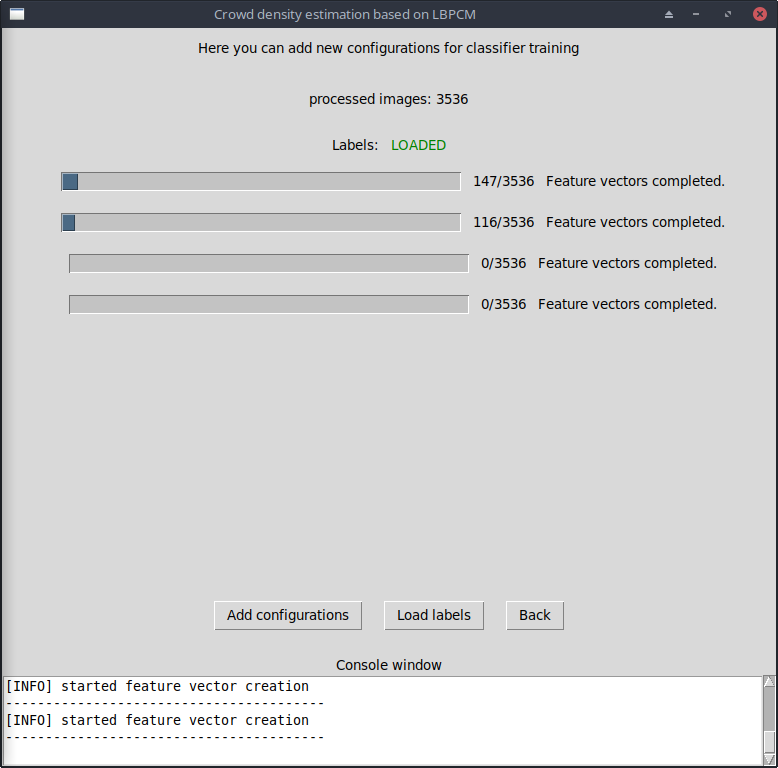
\includegraphics[scale=0.4]{img/fvc3.png}
\captionof{figure}{Prikaz napretka pojedinih konfiguracija}
\end{minipage}

\subsection{Klasifikacija slike postojećim modelima}

Jednom kada je stvaranje vektora značajki završeno i kada je model spremljen 
moguće je pristupiti postupku klasifikacije dosad neviđene slike. 
Kako bi se pristupilo stranici za klasifikaciju potrebno je 
pritisnuti gumb \enquote{Classification} koji se nalazi na glavnoj 
stranici aplikacije. Izgled stranice za klasifikaciju prikazan je na 
slici 4.10.

\begin{minipage}{\linewidth}
\centering
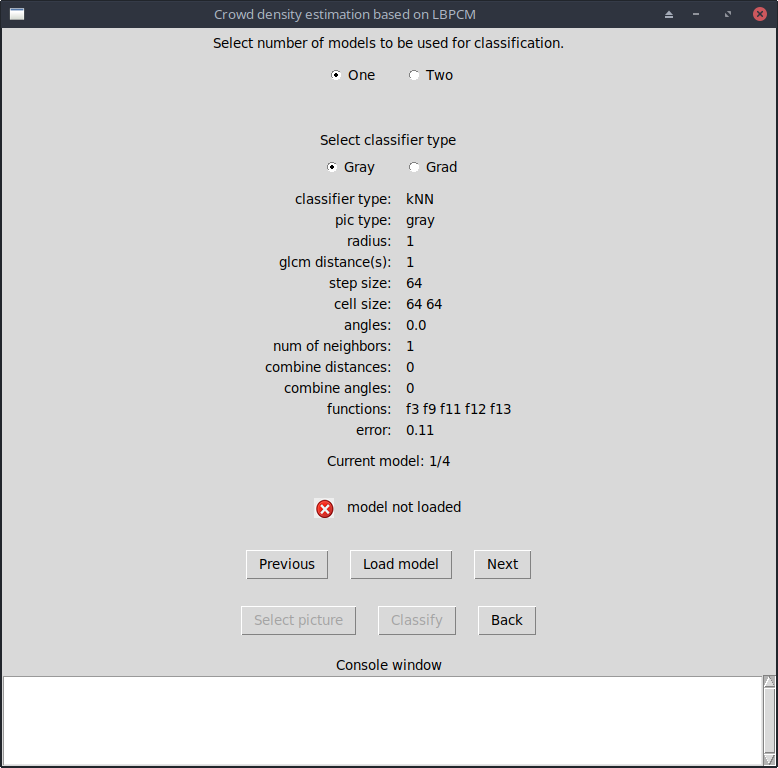
\includegraphics[scale=0.4]{img/cl1.png}
\captionof{figure}{Prikaz stranice za odabir jednog modela}
\end{minipage}

\bigbreak 

Na stranici je prikazana konfiguracija nekog modela koji se nalazi na 
disku računala. Prikazane su sve komponente konkretne konfiguracije
trenutnog modela, a uz to je i prikazana greška klasifikacije pod
nazivom \enquote{error}. Ta greška je omjer točno klasificiranih
podslika i ukupnog broja podslika koji se koristi za testiranje klasifikatora
na podslikama koje nije vidio tijekom faze učenja. 

\bigbreak 

Trenutno je prikazan model koji je učen na slikama sive razine i moguće
je vidjeti da trenutno takvih modela na disku ima 4 (redni broj modela
\enquote{Current model}). Kako bi vidjeli moguće modele koji su učeni na
gradijentnim slikama potrebno je pritisnuti gumb \enquote{Grad}. Za dohvat
sljedećeg ili prethodnog dostupnog modela potrebno je pritisnuti na 
gumbe \enquote{Next} ili \enquote{Previous}. Jednom kada je odabran željeni
model za klasifikaciju potrebno je pritisnuti gumb \enquote{Load model} čime
se prikazani model učitava u memoriju i moguće ga je koristiti za klasifikaciju.
Ako je model ispravno učitan, tekst ispod trenutnog modela se mijenja
u \enquote{model loaded} sa zalenom kvačicom.

\bigbreak

Opisani postupak se primjenjuje kada želimo klasificirati novu sliku
koristeći samo jedan model. U slušaju da želimo koristiti kombinaciju
dva modela potrebno je pritisnuti gumb \enquote{Two} na vrhu stranice.
Nakon pritiska na gumb i učitavanja oba modela izgled stranice je prikazan
na slici 4.11. Jednom učitane modele moguće je koristiti za klasifikaciju. Kako
bi se odabrala željena slika za klasifikaciju potrebno je pritisnuti 
gumb \enquote{Select picture} nakon čega se otvara prozor za odabir slike.
Nakon odabira slike potrebno je pritisnuti na gumb \enquote{Classify} koji 
otvara prozor prikazan na slici 4.12.

\bigbreak 

\begin{minipage}{\linewidth}
\centering
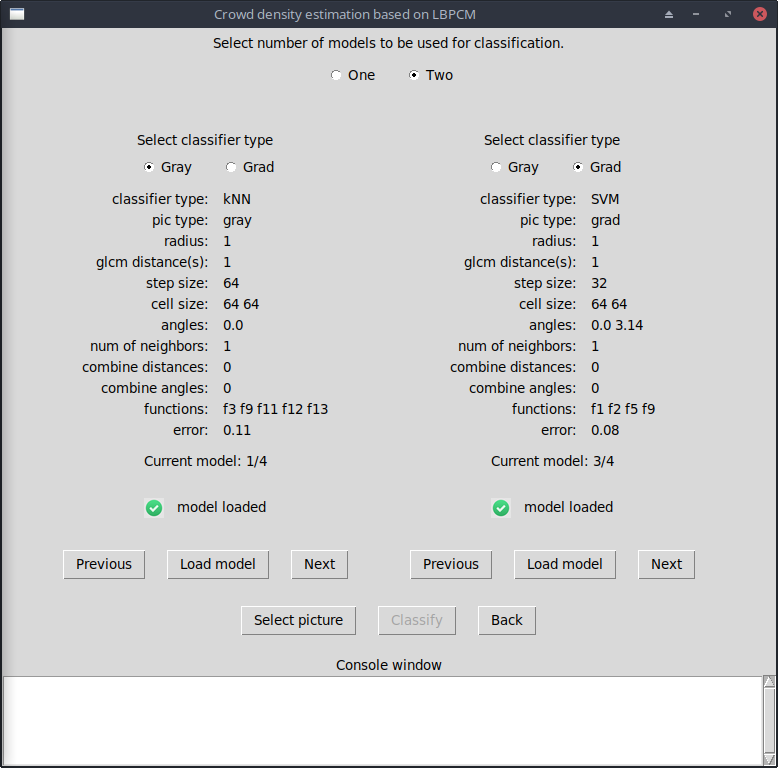
\includegraphics[scale=0.4]{img/cl2.png}
\captionof{figure}{Prikaz stranice za odabir dva modela}
\end{minipage}

\bigbreak

Na slici 4.12. prikazane su 3 identične kopije odabrane slike sljedećeg 
značenja. Na mjestu najveće slike će se prikazati rezultat kombinacije 
obaju modela dok su slike s desne strane rezultati klasifikacije svakog 
pojedinog klasifikatora. 
Razlog za to je uvid u utjecaj pojedinih težina svakog klasifikatora na 
krajnji rezltat klasifikacije. Vrh stranice prikazuje paletu boja koje
su dodijeljene pojedinom razredu gustoće mnoštva radi vizualnog
prikaza rezultata klasifikacije. Klasifikacija se napokon može pokrenuti
pritiskom na gumb \enquote{Start classification} nakon čega je potrebno
pričekati neko vrijeme koje ovisi o složenosti učitanog modela. 

\bigbreak

Podno najveće slike se nakon gotove klasifikacije prikazuje interval
procjene broja ljudi. Ako nije potrebno vidjeti rezultate svakog od
klasifikatora moguće je označiti  \enquote{Only voting classifier}
čime se samo klasificira najveća slika. Jednom kada je klasifikacija 
završila moguće je vidjeti rezultat na slici 4.13.

\bigbreak

\begin{minipage}{\linewidth}
\centering
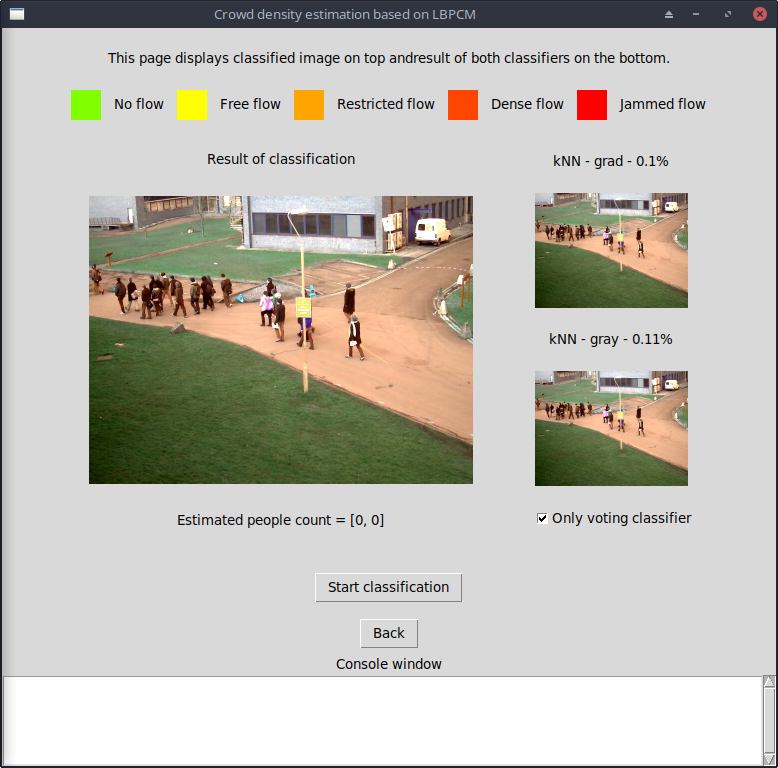
\includegraphics[scale=0.38]{img/cl3.png}
\captionof{figure}{Prikaz stranice za klasifikaciju slika}
\end{minipage}

\bigbreak

\begin{minipage}{\linewidth}
\centering
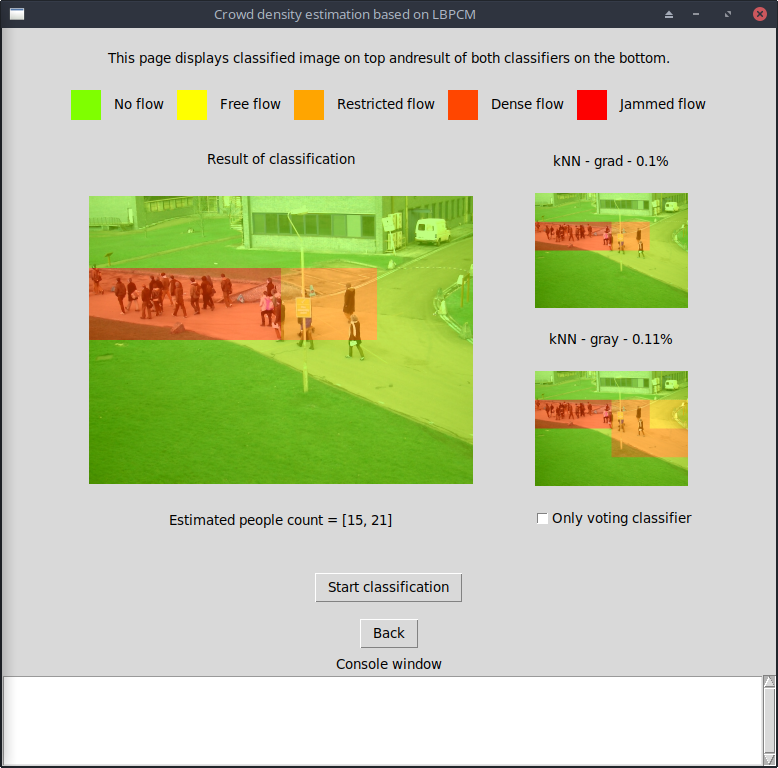
\includegraphics[scale=0.38]{img/cl5.png}
\captionof{figure}{Prikaz klasificirane slike i procjene broja ljudi na 
temelju gustoće mnoštva}
\end{minipage}

\bigbreak

Na slikama koje pokazuju rezultate klasifikacije pojedinih klasifikatora s 
desne strane može se zamijetiti kako točnosti klasifikacije utječu na
krajnji rezultat. Klasifikatori iz primjera nisu najbolje točnosti, 
međutim kada su upareni zajedno, mogu dati bolje rezultate kako je 
i ilustrirano na slici 4.13. To je i cijela ideja korištenja skupnog
klasifikatora koji spaja više njih u jednu cjelinu, u ovom slučaju
dva. 

\bigbreak

Iako se čini iz navedenog primjera da je rezultat samo preslika 
klasifikatora koji ima veću točnost klasifikacije, to ne mora uvijek 
biti slučaj. Nekad može fokus jednog klasifikator biti usmjeren 
na određene dijelove slike koji je možda uvjetovan odabranim 
Haralickovim značajkama, uvjetima osvjetljenja, kutom nagiba kamere ili 
nečim drugim dok drugi klasifikator može imati fokus na sasvim drugi 
dio slike. 

\bigbreak

Opisani problem bi se manifestirao na način da su neka 
područja slike, koja su u fokusu klasifikatora, ispravno klasificirana 
dok druga nisu te jednako tako i za drugi klasifikator, ali kada
su \enquote{spojena} zajedno, daju jedan rezultat koji može davati veoma
dobre rezultate. Pozitivne strane jednog klasifikatora mogu nadjačati 
negativne strane drugog klasifikatora i na kraju rezultirati uspješnom
procjenom gustoće mnoštva. Ta simbioza klasifikatora uvelike je određena 
težinama koje množe pojedine vjerojatnosne vrijednosti svakog klasifikatora.


\chapter{Tehnika klizećeg okna}

Kao jednu od osnovnih alata postupka prikazanog u ovom radu, tehniku
kliznog okna moguće je vidjeti pritiskom na gumb \enquote{Sliding window}
na glavnoj stranici aplikacije. 

\bigbreak

\begin{minipage}{\linewidth}
\centering
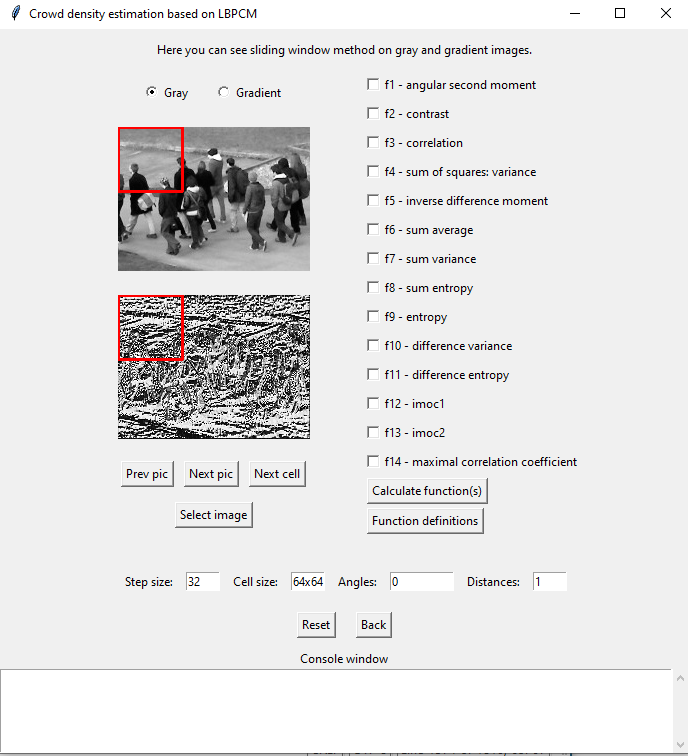
\includegraphics[scale=0.4]{img/sw1.png}
\captionof{figure}{Prikaz prozora tehnike klizećeg okna}
\end{minipage}

\bigbreak

Na slici 5.1. prikazane s dvije podslike koje su izravno učitane iz direktorija
s već obrađenim podslikama za ilustraciju postupka. Ako želimo učitati neku
specifičnu podsliku, to je moguće učiniti pritiskom na gumb \enquote{Select Image}
nakon čega se otvara prozor za odabir željene podslike.

\bigbreak

Vrh prozora omogućava primjenu postupka nad podslikama sive razine i nad slikama
na koje se primijeni operator gradijenta. Za promjenu iz jednog stanja u
drugo potrebno je samo pritisnuti na željeni gumb. Za pomicanje okna na sljedeću
poziciju zaslužan je gumb \enquote{Next cell}. Sljedeća slika iz 
direktorija obrađenih podslika dohvaća se pritiskom na gumb \enquote{Next pic}, a 
prethodna gumbom \enquote{Prev pic}. Podnožje prozora zaokupljaju 
područja za upis parametara vezanih uz LBP i GLCM. 

\bigbreak

Želimo li izračunati vrijednosti konkretnih Haralickovih značajki 
trenutnog okna potrebno je odabrati sve željene značajke u desnom dijelu
prozora te pritisnuti gumb \enquote{Calculate funciton(s)}. Ukoliko
nije jasno kako su neke značajke definirane, moguće je vidjeti njihov
algebarski zapis pritiskom na gumb \enquote{Function definitions}. 
Nakon pritiska na gumb za izračun Haralickovih značajki, njihove vrijednosti
se pojavljuju u konzoli aplikacije. 

\bigbreak

Pogledom u izračune različitih Haralickovih značajki vrijednosti funkcija 
se razlikuju u nekoliko redova veličina stoga ih je potrebno normalizirati
prije nego se vektori značajki predaju klasifikatoru. Normalizacija
je nužan postupak iz razloga što klasifikator koristi mjeru udaljenosti
kao funkciju koja određuje pripadnosti nekom razredu te ako bi ostavili 
vrijednosti ovakvima, neke od njih uopće ne bi imale kikakvog utjecaja zbog 
svoje veličine dok bi druge, koje su možda manje važne u nekim slučajevima,
dominirale i previše utjecale na krajnji rezultat klasifikacije. 

\bigbreak

Normalizacijom se vektori značajki svode na srednju vrijednost oko 0
i jediničnu varijancu.

\bigbreak

Postupak normalizacije:
\begin{center}

N - ukupan broj vektora značajki, \(k\) - k-ta komponenta vektora značajki

\begin{enumerate}
\item Izračun srednje vrijednosti svake komponente vektora značajki
\[
x_k = \frac{1}{N}\sum_{i=1}^{N}x_{ik}
\]

\item Izračun standardne devijacije svake komponente vektora značajki
\[
\sigma_k^2 = \frac{1}{N-1}\sum_{i=1}^N\left(x_{ik}-x_k\right)^2
\]

\item Od vrijednosti svake komponente vektora značajki se oduzme srednja
vrijednost te koponente i podijeli drugim korijenom iz srednje vrijednosti
devijacije te komponente

\[
x_{ik} = \frac{x_{ik}}{\sigma_k}
\]

\end{enumerate}
\end{center}

Nakon postupka normalizacije svi vektori imaju srednje vrijednosti oko nule
i jediničnu varijancu. 

\bigbreak
\underline{\textbf{Primjer}} Stvaranje vektora značajki
\bigbreak

Kao primjer uzmimo 4 Haralickove značajke: kontrast, energiju, homogenost i entropiju. 

\bigbreak

Uvedimo oznake radi jednostavnijeg prikaza: 
\newline \(X_i,j\) predstavlja vrijednost funkcije kontrasta za \(i\)-ti
kut i \(j\)-tu udaljenost u GLCM
\newline \(Y_{i,j}\) predstavlja vrijednost funkcije energije za \(i\)-ti
kut i \(j\)-tu udaljenost u GLCM
\newline \(Z_{i,j}\) predstavlja vrijednost funkcije homogenosti za \(i\)-ti
kut i \(j\)-tu udaljenost u GLCM
\newline \(W_{i,j}\) predstavlja vrijednost funkcije entropije za \(i\)-ti
kut i \(j\)-tu udaljenost u GLCM

\bigbreak

Ukoliko bi uzeli udaljenost \(d=1\) i kutove \(\frac{\pi}{4}, \frac{\pi}{2}, \pi\)
kao parametre GLCM, vektor značajki jednog okna bi izgledao na sljedeći način:
\bigbreak
Radi jednostavnosti zapisa uvedimo indeks 1 za kut \(\frac{\pi}{4}\), 2 za
\(\frac{\pi}{2}\) i 3 za \(\pi\).

\bigbreak

\(
c = \left(X_{1,1}, X_{2,1}, X_{3,1}, Y_{1,1}, Y_{2,1}, Y_{3,1}, Z_{1,1}, 
Z_{2,1}, Z_{3,1}, W_{1,1}, W_{2,1}, W_{3,1}\right)
\)

\bigbreak

Kada je dobiven vektor značajki jednog okna, taj se vektor doda već postojećem 
vektoru značajki podslike te se postupak ponavalja za svako okno podslike.
\newline
Dimenzionalnost vektora značajki pojedinog okna dobije se umnoškom:

\begin{center}

\(A\) - broj Haralickovih značajki

\(B\) - broj kutova u GLCM

\(C\) - broj različitih udaljenosti u GLCM

\end{center}
\[
n = A \cdot B \cdot C = 4 \cdot 3 \cdot 1 = 12
\]

Broj okna u svakoj podslici može se izračunati prema formuli:

\begin{center}

\(X\) - širina podslike u pikselima
\(Y\) - visina podslike u pikselima
\(d_1\) - širina okna u pikselima
\(d_2\) - visina okna u pikselima
\(t\) - korak okna

\[
N = \left(\left\lfloor\frac{X-d_1}{t}\right\rfloor + 1\right) \cdot
\left(\left\lfloor\frac{Y-d_2}{t}\right\rfloor + 1\right)
\]

Ukupna dimenzionalnost vektora značajki pojedine podslike dobije se umnoškom:

\[
dim = N \cdot n
\]

Za konkretan slučaj s parametrima sa slike 5.1. i korištenim Haralickovim 
značajkama iz primjera iznad, dimenzionalnost vektora značajki bi iznosila:

\[
dim = 15 \cdot 12 = 180
\]

\end{center}


\chapter{Rezultati eksperimenta}
Prikaz rezultata 
\newline
Diskusija o utjecaju značajki na točnost klasifikacije - utjecaj
broja značajki na točnost, ima li smisla koristiti puno različitih značajki,
čime se vrijeme izračuna vektora značajki veoma povećava
\newline
Izdvojiti najbolji/optimalni skup parametara

\chapter{Prikladnost korištenog postupka na drugome skupu podataka}

Naći neki skup podataka na internetu s velikom brojem ljudi.
\newline
Ocijeniti prikladnost postupka na novome skupu podataka.




\chapter{Zaključak}
Zaključak.

\bibliography{literatura}
\bibliographystyle{fer}

\listoffigures

\begin{sazetak}
Sažetak na hrvatskom jeziku.

\kljucnerijeci{Ključne riječi, odvojene zarezima.}
\end{sazetak}

% TODO: Navedite naslov na engleskom jeziku.
\engtitle{Crowd density estimation based on local binary pattern co-occurence matrix}
\begin{abstract}
Abstract.

\keywords{Keywords.}
\end{abstract}

\appendix

\chapter{Teksturne značajke}

Oznake korištene dalje u tekstu:
\bigbreak
\(N_g\) - broj sivih razina
\(p(i,j)\) - \((i,j)\)-ti element normalizirane matrice pojavnosti sivih razina
\bigbreak
\(p_x(i)\) - \(i\)-ti element u matrici marginalnih vjerojatnosti koja je dobivena 
zbrajanjem redaka = \(\sum_{j=1}^{N_g}p(i,j)\)
\bigbreak
\(p_y(j)\) - \(j\)-ti element u matrici marginalnih vjerojatnosti koja je dobivena 
zbrajanjem stupaca = \(\sum_{i=1}^{N_g}p(i,j)\)

\[
p_{x+y}(k)=\sum_{i=1}^{N_g} \sum_{j=1}^{N_g} p(i,j) \;\;\; k=2,3,...,2N_g, \; i+j=k
\]

\[
p_{x-y}(k)=\sum_{i=1}^{N_g} \sum_{j=1}^{N_g} p(i,j) \;\;\; k=0,1,...,N_g-1, \; \left|i-j\right|=k
\]

\[
\sum_i \; \textrm{predstavlja pokratu} \; \sum_{i=1}^{N_g} \; \textrm{,a} \;
\sum_{j} \; \textrm{predstavlja pokratu} \; \sum_{j=1}^{N_g}
\]

\bigbreak
1) Angular second moment:
\[
f_1 = \sum_{i}\sum_{j}p(i,j)^2
\]

2) Contrast:
\[
f_2 = \sum_{n=0}^{N_g-1}n^2 \left( \sum_{i=1}^{N_g}\sum_{j=1}^{N_g}p(i,j) \right), \left| i-j \right| = n
\]

3) Correlation:
\[
f_3 = \frac{\sum_i\sum_j\left(ij\right)p(i,j) - \mu_x\mu_y}{\sigma_x\sigma_y}
\]

4) Sum of squares: variance:
\[
f_4 = \sum_i\sum_j(i-\mu)^2p(i,j)
\]

5) Inverse difference moment:
\[
\sum_i\sum_j \frac{1}{1+(i-j)^2}p(i,j)
\]

6) Sum of average:
\[
f_6 = \sum_{i=2}^{2N_g}ip_{x+y}(i)
\]

7) Sum variance:
\[
f_7 = \sum_{i=2}^{2N_g}(i-f_8)^2p_{x+y}(i)
\]

8) Sum entropy:
\[
f_8 = -\sum_{i=2}^{2N_g}p_{x+y}(i)\log(p_{x+y}(i))
\]

9) Entropy:
\[
f_9 = -\sum_i\sum_j p(i,j)\log(p(i,j))
\]

10) Difference variance
\[
f_{10} = \textrm{variance of} \; p_{x-y}
\]

11) Difference entropy:
\[
f_{11} = -\sum_{i=0}^{N_g-1}p_{x-y}(i)\log(p_{x-y}(i)) 
\]

12), 13) Information measures of correlation
\[
f_{12} = \frac{HXY - HXY1}{max\{HX,HY\}}
\]
\[
f_{13} = \sqrt{(1-\exp{-2(HXY2 - HXY)}}
\]
\[
HX = -\sum_i\sum_j p(i,j)\log(p(i,j))
\]
\[
HXY1 = -\sum_i\sum_j p(i,j)\log(p_x(i)p_y(y))
\]
\[
HXY2 = -\sum_i\sum_j p_x(i)p_y(y) \log(p_x(i)p_y(y))
\]

14) Maximal correlation coefficient:
\[
f_{14} = \sqrt{Second \; largest \; eigenvalue \; of \; Q}
\]
\[
Q(i,j) = \sum_k \frac{p(i,k)p(j,k)}{p_x(i)p_y(k)}
\]

\chapter{Rezultati eksperimenta}


\begin{adjustwidth}{-30pt}{0pt}
\begin{tabular}{c|c|c|c|c|c|c|c|c|c|c}
\hline
\STAB{\rotatebox[origin=c]{90}{redni broj}} & 
\STAB{\rotatebox[origin=c]{90}{\;\;vrsta klasifikatora\;\;}} & 
\STAB{\rotatebox[origin=c]{90}{vrsta podslike}} & 
\STAB{\rotatebox[origin=c]{90}{radijus}} & 
\STAB{\rotatebox[origin=c]{90}{GLCM udaljenosti}} & 
\STAB{\rotatebox[origin=c]{90}{korak okna}} & 
\STAB{\rotatebox[origin=c]{90}{veličina okna}} & 
\STAB{\rotatebox[origin=c]{90}{kutovi}} & 
\STAB{\rotatebox[origin=c]{90}{broj susjeda }}& 
\STAB{\rotatebox[origin=c]{90}{značajke}} & 
\STAB{\rotatebox[origin=c]{90}{greška}} \\
\hline
1 & \textit{k}-NN & grad & 1 & 1 & 32 & 64x64 & 0,\(\pi\)& 1 & f1,f2,f5,f9 & 9.9\% \\
2 & SVM & gray & 1 & 1 & 32 & 64x64 & 0,\(\pi\)& - & f1,f2,f5,f9 & 8.86\% \\
3 & SVM & grad & 1 & 1 & 32 & 64x64 & 0,\(\pi\)& - & f1,f2,f5,f9 & 7.92\% \\
4 & \textit{k}-NN & gray & 1 & 1 & 32 & 64x64 & 0,\(\pi\)& 1 & f1,f2,f5,f9 & 9.52\% \\
5 & SVM & gray & 1 & 1 & 32 & 64x64 & 0,\(\pi\)& - & f1,f2,f3,f4,f5,f9 & 8.39\% \\
6 & SVM & grad & 1 & 1 & 32 & 64x64 & 0,\(\pi\)& - & f1,f2,f3,f4,f5,f9 & 8.11\% \\
7 & \textit{k}-NN & grad & 1 & 1 & 32 & 64x64 & 0,\(\pi\)& 3 & f1,f2,f3,f4,f5,f9 & 8.58\% \\
8 & \textit{k}-NN & gray & 1 & 1 & 32 & 64x64 & 0,\(\pi\)& 3 & f1,f2,f3,f4,f5,f9 & 7.45\% \\
9 & SVM & grad & 1 & 1 & 32 & 64x64 & 0,\(\pi\)& - & f8,f9,f12,f13 & 9.99\% \\
10 & \textit{k}-NN & grad & 1 & 1 & 32 & 64x64 & 0,\(\pi\)& 3 & f8,f9,f12,f13 & 11.31\% \\
11 & \textit{k}-NN & gray & 1 & 1 & 32 & 64x64 & 0,\(\pi\)& 3 & f8,f9,f12,f13 & 9.24\% \\
12 & SVM & gray & 1 & 1 & 32 & 64x64 & 0,\(\pi\)& - & f8,f9,f12,f13 & 8.95\% \\
13 & SVM & gray & 1 & 1 & 32 & 64x64 & \(0, \frac{\pi}{2}, \pi, \frac{3\pi}{2}\)& - & f4,f5,f9,f11 & 7.35\% \\
14 & \textit{k}-NN & gray & 1 & 1 & 32 & 64x64 & \(0, \frac{\pi}{2}, \pi, \frac{3\pi}{2}\)& 3 & f4,f5,f9,f11 & 6.79\% \\
15 & \textit{k}-NN & grad & 1 & 1 & 32 & 64x64 & \(0, \frac{\pi}{2}, \pi, \frac{3\pi}{2}\)& 3 & f4,f5,f9,f11 & 7.45\% \\
16 & SVM & grad & 1 & 1 & 32 & 64x64 & \(0, \frac{\pi}{2}, \pi, \frac{3\pi}{2}\)& - & f4,f5,f9,f11 & 8.58\% \\
17 & \textit{k}-NN & grad & 1 & 1 & 64 & 64x64 & \(0, \pi\)& 3 & f9,f10,f11,f12,f13 & 11.12\% \\
18 & SVM & gray & 1 & 1 & 64 & 64x64 & \(0, \pi\)& - & f9,f10,f11,f12,f13 & 10.08\% \\
19 & SVM & grad & 1 & 1 & 64 & 64x64 & \(0, \pi\)& - & f9,f10,f11,f12,f13 & 9.9\% \\

\end{tabular}
\end{adjustwidth}

\newpage

\begin{table}[ht]
\begin{adjustwidth}{-30pt}{0pt}
\begin{tabular}{c|c|c|c|c|c|c|c|c|c|c}
20 & \textit{k}-NN & gray & 1 & 1 & 64 & 64x64 & \(0, \pi\)& 1 & f9,f10,f11,f12,f13 & 10.65\% \\
21 & SVM & grad & 1 & 1 & 32 & 64x64 & 0 & - & f1,f2,f4,f7,f10,f12,f13 & 8.95\% \\
22 & SVM & gray & 1 & 1 & 32 & 64x64 & 0 & - & f1,f2,f4,f7,f10,f12,f13 & 7.82\% \\
23 & SVM & gray & 1 & 1 & 32 & 64x64 & 0, \(\pi\) & - & f1,f2,f4,f7,f10,f12,f13 & 7.82\% \\
24 & SVM & grad & 1 & 1 & 32 & 64x64 & 0, \(\pi\) & - & f1,f2,f4,f7,f10,f12,f13 & 8.95\% \\
25 & SVM & grad & 1 & 1 & 32 & 64x64 & \(0, \frac{\pi}{2}, \pi, \frac{3\pi}{2}\) & - & f1,f2,f3,f4,f5,f9 & 8.77\% \\
26 & SVM & gray & 1 & 1 & 32 & 64x64 & \(0, \frac{\pi}{2}, \pi, \frac{3\pi}{2}\) & - & f1,f2,f3,f4,f5,f9 & 8.29\% \\
27 & SVM & gray & 1 & 1 & 32 & 64x64 & \(0, \frac{\pi}{2}, \pi, \frac{3\pi}{2}\) & - & f1,f2,f3,f4,f5,f9,f12,f13 & 8.2\% \\
28 & SVM & grad & 1 & 1 & 32 & 64x64 & \(0, \frac{\pi}{2}, \pi, \frac{3\pi}{2}\) & - & f1,f2,f3,f4,f5,f9,f12,f13 & 8.58\% \\
29 & SVM & grad & 1 & 1 & 64 & 64x64 & 0 & - & f2,f6,f7,f8,f9 & 8.58\% \\
30 & SVM & gray & 1 & 1 & 64 & 64x64 & 0 & - & f2,f6,f7,f8,f9 & 8.58\% \\
31 & SVM & gray & 1 & 1 & 32 & 64x64 & 0 & - & f2,f6,f7,f8,f9 & 7.73\% \\
32 & SVM & grad & 1 & 1 & 32 & 64x64 & 0 & - & f2,f6,f7,f8,f9 & 8.95\% \\
32 & SVM & grad & 1 & 1 & 32 & 64x64 & 0 & - & f2,f6,f7,f8,f9 & 8.95\% \\
32 & SVM & grad & 1 & 1 & 32 & 64x64 & 0 & - & f2,f6,f7,f8,f9 & 8.95\% \\
32 & SVM & grad & 1 & 1 & 32 & 64x64 & 0 & - & f2,f6,f7,f8,f9 & 8.95\% \\
\end{tabular}
\end{adjustwidth}
\caption{Prikaz rezultata različitih modela klasifikatora} 
\end{table}




\end{document}




